\section{Instance level transformations}
\label{sec:library_of_transformations:instance_level_transformations}

The previous section has presented a set of model transformations between type models and type graphs. In this section, these transformations are used to define model transformations between instance model and instance graphs. Therefore, this section provides the second set of model transformations introduced within the introduction of this chapter. 

Throughout this section, small transformations between instance models and instance graphs will be defined. In order for these transformations useful in the context of the transformation framework of \cref{chapter:transformation_framework}, some properties must hold for each of them. For each transformation, the corresponding instance model and instance graph must be valid in the sense of \cref{defin:formalisations:ecore_formalisation:instance_models:model_validity} and \cref{defin:formalisations:groove_formalisation:instance_graphs:instance_graph_validity} respectively. Furthermore, the instance model corresponding to the transformation must be compatible with its counterpart in the transformation framework. In the same way, the corresponding instance graph must be compatible with its counterpart in the transformation framework. Moreover, it will be shown that the transformation function $f$ that transforms the corresponding instance model into an instance graph is a valid transformation function in the sense of \cref{defin:transformation_framework:instance_models_and_instance_graphs:combining_transformation_functions:transformation_function_instance_model_instance_graph}. Finally, it will also be shown that the reverse transformation is a valid transformation function in the sense of \cref{defin:transformation_framework:instance_models_and_instance_graphs:combining_transformation_functions:transformation_function_instance_graph_instance_model}.

\subsection{Plain objects}
\label{subsec:library_of_transformations:instance_level_transformations:plain_objects}

\begin{figure}[b]
    \centering
    \begin{subfigure}{0.45\textwidth}
        \centering
        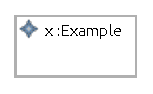
\includegraphics{images/05_library_of_transformations/03_instance_level_transformations/01_plain_objects/class_instance.pdf}
        \caption{$Im_{Class}$ with one object identified as $x$}
        \label{fig:library_of_transformations:instance_level_transformations:plain_objects:visualisation:ecore}
    \end{subfigure}
    \begin{subfigure}{0.45\textwidth}
        \centering
        % To use this figure in your LaTeX document
% import the package groove/resources/groove2tikz.sty
%
\begin{tikzpicture}[scale=\tikzscale,name prefix=start-]
\node[basic_node] (n0) at (1.620, -0.370) {\ml{\uline{\textit{x}} : \textbf{Example}}};

\end{tikzpicture}

        \caption{$IG_{Class}$ with one node identified as $x$}
        \label{fig:library_of_transformations:instance_level_transformations:plain_objects:visualisation:groove}
    \end{subfigure}
    \caption{Visualisation of the transformation of plain objects typed by regular classes}
    \label{fig:library_of_transformations:instance_level_transformations:plain_objects:visualisation}
\end{figure}

The first transformation that will be defined is a transformation of plain objects of a regular class type. The corresponding type level transformation can be found in \cref{subsec:library_of_transformations:type_level_transformations:regular_classes}. This transformation introduces an arbitrary amount of instances of the class introduced on the type level. First, the definition of the corresponding instance model is given.

\begin{defin}[Instance model $Im_{Class}$]
\label{defin:library_of_transformations:instance_level_transformations:plain_objects:imod_class}
Let $Im_{Class}$ be the instance model containing a set of objects $objects$ which are all typed by class $name$. Furthermore, an injective function $fid$ is defined which maps every object in the set to its corresponding identifier. $Im_{Class}$ is typed by $Tm_{Class}$ (\cref{defin:library_of_transformations:type_level_transformations:regular_classes:tmod_class}) and is defined as:
\begin{align*}
Object =\ &objects \\
\mathrm{ObjectClass} =\ & \begin{cases}
    (ob, name) & \mathrm{if }\ ob \in objects
\end{cases}\\
\mathrm{ObjectId} =\ & \begin{cases}
    (ob, fid(ob)) & \mathrm{if }\ ob \in objects
\end{cases}\\
\mathrm{FieldValue} =\ & \{\} \\
\mathrm{DefaultValue} =\ & \{\}
\end{align*}
\isabellelref{imod_class}{Ecore-GROOVE-Mapping-Library.ClassInstance}
\end{defin}

\begin{thm}[Correctness of $Im_{Class}$]
\label{defin:library_of_transformations:instance_level_transformations:plain_objects:imod_class_correct}
$Im_{Class}$ (\cref{defin:library_of_transformations:instance_level_transformations:plain_objects:imod_class}) is a valid instance model in the sense of \cref{defin:formalisations:ecore_formalisation:instance_models:model_validity}.
\isabellelref{imod_class_correct}{Ecore-GROOVE-Mapping-Library.ClassInstance}
\end{thm}

A visual representation of $Im_{Class}$ with $objects = \{ob\}$ and $fid(ob) = x$ can be seen in \cref{fig:library_of_transformations:instance_level_transformations:plain_objects:visualisation:ecore}. Although this visualisation only shows one object, it is possible to have an arbitrary amount of objects in $Im_{Class}$, as long as they are all typed by the corresponding class introduced on the type level. In the visualisation, the identifier $.\type{Example}$ is used for the class, in correspondence with \cref{fig:library_of_transformations:type_level_transformations:regular_classes:visualisation:ecore} The correctness proof of $Im_{Class}$ is trivial, and therefore not included here. The proof can be found as part of the Isabelle validated proofs.

In order to make composing transformation functions possible, $Im_{Class}$ should be compatible with the instance model it is combined with.

\begin{thm}[Correctness of $\mathrm{combine}(Im, Im_{Class})$]
\label{defin:library_of_transformations:instance_level_transformations:plain_objects:imod_class_combine_correct}
Assume an instance model $Im$ that is valid in the sense of \cref{defin:formalisations:ecore_formalisation:instance_models:model_validity}. Then $Im$ is compatible with $Im_{Class}$ (in the sense of \cref{defin:transformation_framework:instance_models_and_instance_graphs:combining_instance_models:compatibility}) if:
\begin{itemize}
    \item All requirements of \cref{defin:library_of_transformations:type_level_transformations:regular_classes:tmod_class_combine_correct} are met, to ensure the combination of the corresponding type models is valid;
    \item All the objects in $Im_{Class}$ have an (internal and explicit) identity that is not yet used in $Im$.
\end{itemize}
\isabellelref{imod_class_combine_correct}{Ecore-GROOVE-Mapping-Library.ClassInstance}
\end{thm}

\begin{proof}
Use \cref{defin:transformation_framework:instance_models_and_instance_graphs:combining_instance_models:imod_combine_merge_correct}. It is possible to show that all assumptions hold. Now we have shown that $\mathrm{combine}(Im, Im_{Class})$ is consistent in the sense of \cref{defin:formalisations:ecore_formalisation:instance_models:model_validity}.
\end{proof}

Please note that this combination is quite trivial, as the newly introduced objects cannot have fields. This is because they are all typed by the new class type introduced in $Tm_{Class}$. Since this new class type is new by assumption, the existing model cannot have fields defined for the class type.

The definitions and theorems for introducing plain objects of regular classes within Ecore are now complete. 

\subsubsection{Encoding as nodes}

A possible encoding for plain objects in Ecore is using nodes in GROOVE. Each node is typed by the node type that was introduced in $TG_{Class}$, and copies the identifiers set of the objects to the corresponding nodes. The encoding corresponding to $Im_{Class}$ can then be represented as $IG_{Class}$, defined in the following definition:

\begin{defin}[Instance graph $IG_{Class}$]
\label{defin:library_of_transformations:instance_level_transformations:plain_objects:ig_class_as_node_type}
Let $IG_{Class}$ be the instance graph with as nodes the converted $objects$ of $Im_{Class}$ (\cref{defin:library_of_transformations:instance_level_transformations:plain_objects:imod_class}). Furthermore, reuse the injective function $fid$ that maps every object to its identifier. Finally, use the node type introduced in $TG_{Class}$ (\cref{defin:library_of_transformations:type_level_transformations:regular_classes:tg_class_as_node_type}). $IG_{Class}$ is defined typed by $TG_{Class}$ and is defined as:
\begin{align*}
N =\ & objects \\
E =\ & \{\} \\
\mathrm{ident} =\ & \begin{cases}
    (fid(ob), ob) & \mathrm{if }\ ob \in objects
\end{cases}
\end{align*}
with
\begin{align*}
\mathrm{type}_n =\ & \begin{cases}
    (ob, \mathrm{ns\_\!to\_\!list}(name)) & \mathrm{if }\ ob \in objects
\end{cases}
\end{align*}
\isabellelref{ig_class_as_node_type}{Ecore-GROOVE-Mapping-Library.ClassInstance}
\end{defin}

\begin{thm}[Correctness of $IG_{Class}$]
\label{defin:library_of_transformations:instance_level_transformations:plain_objects:ig_class_as_node_type_correct}
$IG_{Class}$ (\cref{defin:library_of_transformations:instance_level_transformations:plain_objects:ig_class_as_node_type}) is a valid instance graph in the sense of \cref{defin:formalisations:groove_formalisation:instance_graphs:instance_graph_validity}.
\isabellelref{ig_class_as_node_type_correct}{Ecore-GROOVE-Mapping-Library.ClassInstance}
\end{thm}

A visual representation of $IG_{Class}$ with $objects = \{ob\}$ and $fid(ob) = x$ can be seen in \cref{fig:library_of_transformations:instance_level_transformations:plain_objects:visualisation:groove}. Like the previous example for the Ecore instance model, only one node is shown here, but multiple nodes can be introduced at once if there are more objects in the $objects$ set. As shown in the definition, the node type identified by $\type{Example}$ is used to type all the nodes, in correspondence with \cref{fig:library_of_transformations:type_level_transformations:regular_classes:visualisation:groove}. The correctness proof of $IG_{Class}$ is trivial, and therefore not included here. The proof can be found as part of the Isabelle validated proofs.

In order to make composing transformation functions possible, $IG_{Class}$ should be compatible with the instance graph it is combined with.

\begin{thm}[Correctness of $\mathrm{combine}(IG, IG_{Class})$]
\label{defin:library_of_transformations:instance_level_transformations:plain_objects:ig_class_as_node_type_combine_correct}
Assume an instance graph $IG$ that is valid in the sense of \cref{defin:formalisations:groove_formalisation:instance_graphs:instance_graph_validity}. Then $IG$ is compatible with $IG_{Class}$ (in the sense of \cref{defin:transformation_framework:instance_models_and_instance_graphs:combining_instance_graphs:compatibility}) if:
\begin{itemize}
    \item All requirements of \cref{defin:library_of_transformations:type_level_transformations:regular_classes:tg_class_as_node_type_combine_correct} are met, to ensure the combination of the corresponding type graphs is valid;
    \item All the nodes in $IG_{Class}$ have an (internal and explicit) identity that is not yet used in $IG$.
\end{itemize}
\isabellelref{ig_class_as_node_type_combine_correct}{Ecore-GROOVE-Mapping-Library.ClassInstance}
\end{thm}

\begin{proof}
Use \cref{defin:transformation_framework:instance_models_and_instance_graphs:combining_instance_graphs:ig_combine_merge_correct}. It is possible to show that all assumptions hold. Now we have shown that $\mathrm{combine}(IG, IG_{Class})$ is valid in the sense of \cref{defin:formalisations:groove_formalisation:instance_graphs:instance_graph_validity}.
\end{proof}

The next definitions define the transformation function from $Im_{Class}$ to $IG_{Class}$:

\begin{defin}[Transformation function $f_{Class}$]
\label{defin:library_of_transformations:instance_level_transformations:plain_objects:imod_class_to_ig_class_as_node_type}
The transformation function $f_{Class}(Im)$ is defined as:
\begin{align*}
N =\ & Object_{Im} \\
E =\ & \{\} \\
\mathrm{ident} =\ & \begin{cases}
    (fid(ob), ob) & \mathrm{if }\ ob \in Object_{Im}
\end{cases}
\end{align*}
with
\begin{align*}
\mathrm{type}_n =\ & \begin{cases}
    (ob, \mathrm{ns\_\!to\_\!list}(name)) & \mathrm{if }\ ob \in Object_{Im}
\end{cases}
\end{align*}
\isabellelref{imod_class_to_ig_class_as_node_type}{Ecore-GROOVE-Mapping-Library.ClassInstance}
\end{defin}

\begin{thm}[Correctness of $f_{Class}$]
\label{defin:library_of_transformations:instance_level_transformations:plain_objects:imod_class_to_ig_class_as_node_type_func}
$f_{Class}(Im)$ (\cref{defin:library_of_transformations:instance_level_transformations:plain_objects:imod_class_to_ig_class_as_node_type}) is a valid transformation function in the sense of \cref{defin:transformation_framework:instance_models_and_instance_graphs:combining_transformation_functions:transformation_function_instance_model_instance_graph} transforming $Im_{Class}$ into $IG_{Class}$.
\isabellelref{imod_class_to_ig_class_as_node_type_func}{Ecore-GROOVE-Mapping-Library.ClassInstance}
\end{thm}

The proof of the correctness of $f_{Class}$ will not be included here. Instead, it can be found in the validated Isabelle theories. The proof is quite trivial, as extending $Im$ can only add extra objects, but not remove the existing ones.

Finally, to complete the transformation, the transformation function that transforms $IG_{Class}$ into $Im_{Class}$ is defined:

\begin{defin}[Transformation function $f'_{Class}$]
\label{defin:library_of_transformations:instance_level_transformations:plain_objects:ig_class_as_node_type_to_imod_class}
The transformation function $f'_{Class}(IG)$ is defined as:
\begin{align*}
Object =\ &N_{IG} \\
\mathrm{ObjectClass} =\ & \begin{cases}
    (ob, name) & \mathrm{if }\ ob \in N_{IG}
\end{cases}\\
\mathrm{ObjectId} =\ & \begin{cases}
    (ob, fid(ob)) & \mathrm{if }\ ob \in N_{IG}
\end{cases}\\
\mathrm{FieldValue} =\ & \{\} \\
\mathrm{DefaultValue} =\ & \{\}
\end{align*}
\isabellelref{ig_class_as_node_type_to_imod_class}{Ecore-GROOVE-Mapping-Library.ClassInstance}
\end{defin}

\begin{thm}[Correctness of $f'_{Class}$]
\label{defin:library_of_transformations:instance_level_transformations:plain_objects:ig_class_as_node_type_to_tmod_class_func}
$f'_{Class}(IG)$ (\cref{defin:library_of_transformations:instance_level_transformations:plain_objects:ig_class_as_node_type_to_imod_class}) is a valid transformation function in the sense of \cref{defin:transformation_framework:instance_models_and_instance_graphs:combining_transformation_functions:transformation_function_instance_graph_instance_model} transforming $IG_{Class}$ into $Im_{Class}$.
\isabellelref{ig_class_as_node_type_to_imod_class_func}{Ecore-GROOVE-Mapping-Library.ClassInstance}
\end{thm}

Once more, the correctness proof is not included here but can be found in the validated Isabelle proofs of this thesis.
\subsection{Abstract classes}
\label{subsec:library_of_transformations:instance_level_transformations:abstract_classes}

In this section, the instance level transformation corresponding to the type level transformation of abstract classes is discussed. The type level transformation of abstract class types can be found in \cref{subsec:library_of_transformations:type_level_transformations:abstract_classes}.

Informally speaking, it is quite weird to think about the transformation of abstract classes on the instance level, as abstract classes cannot have instances. The transformation here is included for completeness, to allow for adding abstract types while working with transformations on the type level. In practice, the instance level will consist of the empty instance model and empty instance graph, showing that after adding an abstract class on the type level, instances of the type model will still be valid.

First, the corresponding instance model is introduced.

\begin{defin}[Instance model $Im_{AbsClass}$]
\label{defin:library_of_transformations:instance_level_transformations:abstract_classes:imod_abstract_class}
Let $Im_{AbsClass}$ be the empty instance model $Im_\epsilon$ (\cref{defin:transformation_framework:instance_models_and_instance_graphs:combining_instance_models:empty_instance_model}), except that it is typed by the type model $Tm_{AbsClass}$ (\cref{defin:library_of_transformations:type_level_transformations:abstract_classes:tmod_abstract_class}).
\isabellelref{imod_abstract_class}{Ecore-GROOVE-Mapping-Library.AbstractClassInstance}
\end{defin}

\begin{thm}[Correctness of $Im_{AbsClass}$]
\label{defin:library_of_transformations:instance_level_transformations:abstract_classes:imod_abstract_class_correct}
$Im_{AbsClass}$ (\cref{defin:library_of_transformations:instance_level_transformations:abstract_classes:imod_abstract_class}) is a valid instance model in the sense of \cref{defin:formalisations:ecore_formalisation:instance_models:model_validity}.
\isabellelref{imod_abstract_class_correct}{Ecore-GROOVE-Mapping-Library.AbstractClassInstance}
\end{thm}

Since $Im_{AbsClass}$ does not define any objects, there is no need for a visual representation. However, in order to make composing transformation functions possible, $Im_{AbsClass}$ should still be compatible with the instance model it is combined with.

\begin{thm}[Correctness of $\mathrm{combine}(Im, Im_{AbsClass})$]
\label{defin:library_of_transformations:instance_level_transformations:abstract_classes:imod_abstract_class_combine_correct}
Assume an instance model $Im$ that is valid in the sense of \cref{defin:formalisations:ecore_formalisation:instance_models:model_validity}. Then $Im$ is compatible with $Im_{AbsClass}$ (in the sense of \cref{defin:transformation_framework:instance_models_and_instance_graphs:combining_instance_models:compatibility}) if:
\begin{itemize}
    \item All requirements of \cref{defin:library_of_transformations:type_level_transformations:abstract_classes:tmod_abstract_class_combine_correct} are met, to ensure the combination of the corresponding type models is valid.
\end{itemize}
\isabellelref{imod_abstract_class_combine_correct}{Ecore-GROOVE-Mapping-Library.AbstractClassInstance}
\end{thm}

\begin{proof}
Use \cref{defin:transformation_framework:instance_models_and_instance_graphs:combining_instance_models:imod_combine_merge_correct}. It is possible to show that all assumptions hold. Now we have shown that $\mathrm{combine}(Im, Im_{AbsClass})$ is consistent in the sense of \cref{defin:formalisations:ecore_formalisation:instance_models:model_validity}.
\end{proof}

The definitions and theorems for the Ecore instance model corresponding to $Tm_{AbsClass}$ are now complete. 

\subsubsection{The node type encoding}

As has been shown earlier, an possible encoding for abstract class types is by introducing an abstract node type. This has been done in $TG_{AbsClass}$. Like the Ecore instance model, the GROOVE instance graph is also empty, because abstract node types cannot be instantiated. This gives rise to $IG_{AbsClass}$, which is defined as follows:

\begin{defin}[Instance graph $IG_{AbsClass}$]
\label{defin:library_of_transformations:instance_level_transformations:abstract_classes:ig_abstract_class_as_node_type}
Let $IG_{AbsClass}$ be the empty instance graph $IG_\epsilon$ (\cref{defin:transformation_framework:instance_models_and_instance_graphs:combining_instance_graphs:empty_instance_graph}), except that it is typed by the type graph $TG_{AbsClass}$ (\cref{defin:library_of_transformations:type_level_transformations:abstract_classes:tg_abstract_class_as_node_type}).
\isabellelref{ig_abstract_class_as_node_type}{Ecore-GROOVE-Mapping-Library.AbstractClassInstance}
\end{defin}

\begin{thm}[Correctness of $IG_{AbsClass}$]
\label{defin:library_of_transformations:instance_level_transformations:abstract_classes:ig_class_as_node_type_correct}
$IG_{AbsClass}$ (\cref{defin:library_of_transformations:instance_level_transformations:abstract_classes:ig_abstract_class_as_node_type}) is a valid instance graph in the sense of \cref{defin:formalisations:groove_formalisation:instance_graphs:instance_graph_validity}.
\isabellelref{ig_abstract_class_as_node_type_correct}{Ecore-GROOVE-Mapping-Library.AbstractClassInstance}
\end{thm}

In order to make composing transformation functions possible, $IG_{AbsClass}$ should be compatible with the instance graph it is combined with.

\begin{thm}[Correctness of $\mathrm{combine}(IG, IG_{AbsClass})$]
\label{defin:library_of_transformations:instance_level_transformations:abstract_classes:ig_abstract_class_as_node_type_combine_correct}
Assume an instance graph $IG$ that is valid in the sense of \cref{defin:formalisations:groove_formalisation:instance_graphs:instance_graph_validity}. Then $IG$ is compatible with $IG_{AbsClass}$ (in the sense of \cref{defin:transformation_framework:instance_models_and_instance_graphs:combining_instance_graphs:compatibility}) if:
\begin{itemize}
    \item All requirements of \cref{defin:library_of_transformations:type_level_transformations:abstract_classes:tg_abstract_class_as_node_type_combine_correct} are met, to ensure the combination of the corresponding type graphs is valid.
\end{itemize}
\isabellelref{ig_abstract_class_as_node_type_combine_correct}{Ecore-GROOVE-Mapping-Library.AbstractClassInstance}
\end{thm}

\begin{proof}
Use \cref{defin:transformation_framework:instance_models_and_instance_graphs:combining_instance_graphs:ig_combine_merge_correct}. It is possible to show that all assumptions hold. Now we have shown that $\mathrm{combine}(IG, IG_{AbsClass})$ is valid in the sense of \cref{defin:formalisations:groove_formalisation:instance_graphs:instance_graph_validity}.
\end{proof}

The next definitions define the transformation function from $Im_{AbsClass}$ to $IG_{AbsClass}$:

\begin{defin}[Transformation function $f_{AbsClass}$]
\label{defin:library_of_transformations:instance_level_transformations:abstract_classes:imod_abstract_class_to_ig_abstract_class_as_node_type}
The transformation function $f_{AbsClass}(Im)$ is defined as the function that always outputs the empty instance graph $IG_\epsilon$ (\cref{defin:transformation_framework:instance_models_and_instance_graphs:combining_instance_graphs:empty_instance_graph}), except that it is typed by $TG_{AbsClass}$.
\isabellelref{imod_abstract_class_to_ig_abstract_class_as_node_type}{Ecore-GROOVE-Mapping-Library.AbstractClassInstance}
\end{defin}

\begin{thm}[Correctness of $f_{AbsClass}$]
\label{defin:library_of_transformations:instance_level_transformations:abstract_classes:imod_abstract_class_to_ig_abstract_class_as_node_type_func}
$f_{AbsClass}(Im)$ (\cref{defin:library_of_transformations:instance_level_transformations:abstract_classes:imod_abstract_class_to_ig_abstract_class_as_node_type}) is a valid transformation function in the sense of \cref{defin:transformation_framework:instance_models_and_instance_graphs:combining_transformation_functions:transformation_function_instance_model_instance_graph} transforming $Im_{AbsClass}$ into $IG_{AbsClass}$.
\isabellelref{imod_abstract_class_to_ig_abstract_class_as_node_type_func}{Ecore-GROOVE-Mapping-Library.AbstractClassInstance}
\end{thm}

The proof of the correctness of $f_{AbsClass}$ will not be included here. Instead, it can be found in the validated Isabelle theories. Obviously, the proof is trivial, as the function does not do any conversion. It does just output the empty instance model.

Finally, to complete the transformation, the transformation function that transforms $IG_{AbsClass}$ into $Im_{AbsClass}$ is defined:

\begin{defin}[Transformation function $f'_{AbsClass}$]
\label{defin:library_of_transformations:instance_level_transformations:abstract_classes:ig_abstract_class_as_node_type_to_imod_abstract_class}
The transformation function $f'_{AbsClass}(IG)$ is defined as the function that always outputs the empty instance model $Im_\epsilon$ (\cref{defin:transformation_framework:instance_models_and_instance_graphs:combining_instance_models:empty_instance_model}), except that it is typed by $Tm_{AbsClass}$.
\isabellelref{ig_abstract_class_as_node_type_to_imod_abstract_class}{Ecore-GROOVE-Mapping-Library.AbstractClassInstance}
\end{defin}

\begin{thm}[Correctness of $f'_{AbsClass}$]
\label{defin:library_of_transformations:instance_level_transformations:abstract_classes:ig_abstract_class_as_node_type_to_imod_abstract_class_func}
$f'_{AbsClass}(IG)$ (\cref{defin:library_of_transformations:instance_level_transformations:abstract_classes:ig_abstract_class_as_node_type_to_imod_abstract_class}) is a valid transformation function in the sense of \cref{defin:transformation_framework:instance_models_and_instance_graphs:combining_transformation_functions:transformation_function_instance_graph_instance_model} transforming $IG_{AbsClass}$ into $Im_{AbsClass}$.
\isabellelref{ig_abstract_class_as_node_type_to_imod_abstract_class_func}{Ecore-GROOVE-Mapping-Library.AbstractClassInstance}
\end{thm}

Once more, the correctness proof is not included here but can be found in the validated Isabelle proofs of this thesis.
\subsection{Plain objects typed by a subclass}
\label{subsec:library_of_transformations:instance_level_transformations:objects_of_subtype}

\begin{figure}
    \centering
    \begin{subfigure}{0.45\textwidth}
        \centering
        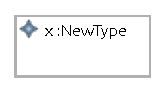
\includegraphics{images/05_library_of_transformations/03_instance_level_transformations/03_objects_of_subtype/subclass_instance.pdf}
        \caption{$Im_{Subclass}$ with one object identified as $x$}
        \label{fig:library_of_transformations:instance_level_transformations:objects_of_subtype:visualisation:ecore}
    \end{subfigure}
    \begin{subfigure}{0.45\textwidth}
        \centering
        % To use this figure in your LaTeX document
% import the package groove/resources/groove2tikz.sty
%
\begin{tikzpicture}[scale=\tikzscale,name prefix=start-]
\node[basic_node] (n0) at (1.620, -0.370) {\ml{\uline{\textit{x}} : \textbf{NewType}}};

\end{tikzpicture}

        \caption{$IG_{Subclass}$ with one node identified as $x$}
        \label{fig:library_of_transformations:instance_level_transformations:objects_of_subtype:visualisation:groove}
    \end{subfigure}
    \caption{Visualisation of the transformation of objects typed by a subclass}
    \label{fig:library_of_transformations:instance_level_transformations:objects_of_subtype:visualisation}
\end{figure}

In this section, the transformation of plain objects typed by a regular subclass is discussed. The corresponding type level transformation can be found in \cref{subsec:library_of_transformations:type_level_transformations:regular_subclasses}. This transformation is very similar to the the transformation of plain objects discussed in \cref{subsec:library_of_transformations:instance_level_transformations:plain_objects}. Like that transformation, it is possible to introduce an arbitrary amount of instances of the subclass introduced on the type level. First, the definition of the corresponding instance model is given.

\begin{defin}[Instance model $Im_{Subclass}$]
\label{defin:library_of_transformations:instance_level_transformations:objects_of_subtype:imod_subclass}
Let $Im_{Subclass}$ be the instance model containing a set of objects $objects$ which are all typed by subclass $name$, which extends class $supertype$. Furthermore, an injective function $fid$ is defined which maps every object in the set to its corresponding identifier. $Im_{Subclass}$ is typed by $Tm_{Subclass}$ (\cref{defin:library_of_transformations:type_level_transformations:regular_subclasses:tmod_subclass}) and is defined as:
\begin{align*}
Object =\ &objects \\
\mathrm{ObjectClass} =\ & \begin{cases}
    (ob, name) & \mathrm{if }\ ob \in objects
\end{cases}\\
\mathrm{ObjectId} =\ & \begin{cases}
    (ob, fid(ob)) & \mathrm{if }\ ob \in objects
\end{cases}\\
\mathrm{FieldValue} =\ & \{\} \\
\mathrm{DefaultValue} =\ & \{\}
\end{align*}
\isabellelref{imod_subclass}{Ecore-GROOVE-Mapping-Library.SubclassInstance}
\end{defin}

\begin{thm}[Correctness of $Im_{Subclass}$]
\label{defin:library_of_transformations:instance_level_transformations:objects_of_subtype:imod_subclass_correct}
$Im_{Subclass}$ (\cref{defin:library_of_transformations:instance_level_transformations:objects_of_subtype:imod_subclass}) is a valid instance model in the sense of \cref{defin:formalisations:ecore_formalisation:instance_models:model_validity}.
\isabellelref{imod_subclass_correct}{Ecore-GROOVE-Mapping-Library.SubclassInstance}
\end{thm}

A visual representation of $Im_{Subclass}$ with $objects = \{ob\}$ and $fid(ob) = x$ can be seen in \cref{fig:library_of_transformations:instance_level_transformations:objects_of_subtype:visualisation:ecore}. Although this visualisation only shows one object, it is possible to have an arbitrary amount of objects in $Im_{Subclass}$, as long as they are all typed by the corresponding class introduced on the type level. In the visualisation, the identifier $.\type{NewType}$ is used for the class, in correspondence with \cref{fig:library_of_transformations:type_level_transformations:regular_subclasses:visualisation:ecore} The correctness proof of $Im_{Subclass}$ is trivial, and therefore not included here. The proof can be found as part of the Isabelle validated proofs.

In order to make composing transformation functions possible, $Im_{Subclass}$ should be compatible with the instance model it is combined with.

\begin{thm}[Correctness of $\mathrm{combine}(Im, Im_{Subclass})$]
\label{defin:library_of_transformations:instance_level_transformations:objects_of_subtype:imod_subclass_combine_correct}
Assume an instance model $Im$ that is valid in the sense of \cref{defin:formalisations:ecore_formalisation:instance_models:model_validity}. Then $Im$ is compatible with $Im_{Subclass}$ (in the sense of \cref{defin:transformation_framework:instance_models_and_instance_graphs:combining_instance_models:compatibility}) if:
\begin{itemize}
    \item All requirements of \cref{defin:library_of_transformations:type_level_transformations:regular_subclasses:tmod_subclass_combine_correct} are met, to ensure the combination of the corresponding type models is valid;
    \item All the objects in $Im_{Subclass}$ have an (internal and explicit) identity that is not yet used in $Im$;
    \item $Im$ is not typed by a type model that defines any fields for the $supertype$ class.
\end{itemize}
\isabellelref{imod_subclass_combine_correct}{Ecore-GROOVE-Mapping-Library.SubclassInstance}
\end{thm}

\begin{proof}
Use \cref{defin:transformation_framework:instance_models_and_instance_graphs:combining_instance_models:imod_combine_merge_correct}. It is possible to show that all assumptions hold. Now we have shown that $\mathrm{combine}(Im, Im_{Subclass})$ is consistent in the sense of \cref{defin:formalisations:ecore_formalisation:instance_models:model_validity}.
\end{proof}

Please note that in this case, it has been made explicit that the new objects introduced do not have any fields defined. This is by ensuring the supertype does not define any fields. The new subclass does not have fields itself, as it cannot have existed in the combined type model.

The definitions and theorems for introducing plain objects of regular subclasses within Ecore are now complete. 

\subsubsection{Encoding as nodes}

As was the case with plain objects of regular classes, a possible encoding for plain objects of subclasses in Ecore is using nodes in GROOVE. Each node is typed by the node type that was introduced in $TG_{Subclass}$, and copies the identifiers set of the objects to the corresponding nodes. The encoding corresponding to $Im_{Subclass}$ can then be represented as $IG_{Subclass}$, defined in the following definition:

\begin{defin}[Instance graph $IG_{Subclass}$]
\label{defin:library_of_transformations:instance_level_transformations:objects_of_subtype:ig_subclass_as_node_type}
Let $IG_{Subclass}$ be the instance graph with as nodes the converted $objects$ of $Im_{Subclass}$ (\cref{defin:library_of_transformations:instance_level_transformations:objects_of_subtype:imod_subclass}). Furthermore, reuse the injective function $fid$ that maps every object to its identifier. Finally, use the node type $name$ introduced in $TG_{Subclass}$, that extends the $supertype$ node type. (\cref{defin:library_of_transformations:type_level_transformations:regular_classes:tg_class_as_node_type}). $IG_{Subclass}$ is defined typed by $TG_{Subclass}$ and is defined as:
\begin{align*}
N =\ & objects \\
E =\ & \{\} \\
\mathrm{ident} =\ & \begin{cases}
    (fid(ob), ob) & \mathrm{if }\ ob \in objects
\end{cases}
\end{align*}
with
\begin{align*}
\mathrm{type}_n =\ & \begin{cases}
    (ob, \mathrm{ns\_\!to\_\!list}(name)) & \mathrm{if }\ ob \in objects
\end{cases}
\end{align*}
\isabellelref{ig_subclass_as_node_type}{Ecore-GROOVE-Mapping-Library.SubclassInstance}
\end{defin}

\begin{thm}[Correctness of $IG_{Subclass}$]
\label{defin:library_of_transformations:instance_level_transformations:objects_of_subtype:ig_subclass_as_node_type_correct}
$IG_{Subclass}$ (\cref{defin:library_of_transformations:instance_level_transformations:objects_of_subtype:ig_subclass_as_node_type}) is a valid instance graph in the sense of \cref{defin:formalisations:groove_formalisation:instance_graphs:instance_graph_validity}.
\isabellelref{ig_subclass_as_node_type_correct}{Ecore-GROOVE-Mapping-Library.SubclassInstance}
\end{thm}

A visual representation of $IG_{Subclass}$ with $objects = \{ob\}$ and $fid(ob) = x$ can be seen in \cref{fig:library_of_transformations:instance_level_transformations:objects_of_subtype:visualisation:groove}. Like the previous example for the Ecore instance model, only one node is shown here, but multiple nodes can be introduced at once if there are more objects in the $objects$ set. As shown in the definition, the node type identified by $\type{NewType}$ is used to type all the nodes, in correspondence with \cref{fig:library_of_transformations:type_level_transformations:regular_subclasses:visualisation:groove}. The correctness proof of $IG_{Subclass}$ is trivial, and therefore not included here. The proof can be found as part of the Isabelle validated proofs.

In order to make composing transformation functions possible, $IG_{Subclass}$ should be compatible with the instance graph it is combined with.

\begin{thm}[Correctness of $\mathrm{combine}(IG, IG_{Subclass})$]
\label{defin:library_of_transformations:instance_level_transformations:objects_of_subtype:ig_subclass_as_node_type_combine_correct}
Assume an instance graph $IG$ that is valid in the sense of \cref{defin:formalisations:groove_formalisation:instance_graphs:instance_graph_validity}. Then $IG$ is compatible with $IG_{Subclass}$ (in the sense of \cref{defin:transformation_framework:instance_models_and_instance_graphs:combining_instance_graphs:compatibility}) if:
\begin{itemize}
    \item All requirements of \cref{defin:library_of_transformations:type_level_transformations:regular_subclasses:tg_subclass_as_node_type_combine_correct} are met, to ensure the combination of the corresponding type graphs is valid;
    \item All the nodes in $IG_{Subclass}$ have an (internal and explicit) identity that is not yet used in $IG$;
    \item There are no edge types from or to the $supertype$ node type, this includes edges from and to types that $supertype$ inherits from.
\end{itemize}
\isabellelref{ig_subclass_as_node_type_combine_correct}{Ecore-GROOVE-Mapping-Library.SubclassInstance}
\end{thm}

\begin{proof}
Use \cref{defin:transformation_framework:instance_models_and_instance_graphs:combining_instance_graphs:ig_combine_merge_correct}. It is possible to show that all assumptions hold. Now we have shown that $\mathrm{combine}(IG, IG_{Subclass})$ is valid in the sense of \cref{defin:formalisations:groove_formalisation:instance_graphs:instance_graph_validity}.
\end{proof}

Like the correctness for the Ecore instance model, validity is guaranteed here by assuming there exist no edge types from and to the $supertype$ node type.

The next definitions define the transformation function from $Im_{Subclass}$ to $IG_{Subclass}$:

\begin{defin}[Transformation function $f_{Subclass}$]
\label{defin:library_of_transformations:instance_level_transformations:objects_of_subtype:imod_subclass_to_ig_subclass_as_node_type}
The transformation function $f_{Subclass}(Im)$ is defined as:
\begin{align*}
N =\ & Object_{Im} \\
E =\ & \{\} \\
\mathrm{ident} =\ & \begin{cases}
    (fid(ob), ob) & \mathrm{if }\ ob \in Object_{Im}
\end{cases}
\end{align*}
with
\begin{align*}
\mathrm{type}_n =\ & \begin{cases}
    (ob, \mathrm{ns\_\!to\_\!list}(name)) & \mathrm{if }\ ob \in Object_{Im}
\end{cases}
\end{align*}
\isabellelref{imod_subclass_to_ig_subclass_as_node_type}{Ecore-GROOVE-Mapping-Library.SubclassInstance}
\end{defin}

\begin{thm}[Correctness of $f_{Subclass}$]
\label{defin:library_of_transformations:instance_level_transformations:objects_of_subtype:imod_subclass_to_ig_subclass_as_node_type_func}
$f_{Subclass}(Im)$ (\cref{defin:library_of_transformations:instance_level_transformations:objects_of_subtype:imod_subclass_to_ig_subclass_as_node_type}) is a valid transformation function in the sense of \cref{defin:transformation_framework:instance_models_and_instance_graphs:combining_transformation_functions:transformation_function_instance_model_instance_graph} transforming $Im_{Subclass}$ into $IG_{Subclass}$.
\isabellelref{imod_subclass_to_ig_subclass_as_node_type_func}{Ecore-GROOVE-Mapping-Library.SubclassInstance}
\end{thm}

The proof of the correctness of $f_{Subclass}$ will not be included here. Instead, it can be found in the validated Isabelle theories. The proof is quite trivial, as extending $Im$ can only add extra objects, but not remove the existing ones.

Finally, to complete the transformation, the transformation function that transforms $IG_{Subclass}$ into $Im_{Subclass}$ is defined:

\begin{defin}[Transformation function $f'_{Subclass}$]
\label{defin:library_of_transformations:instance_level_transformations:objects_of_subtype:ig_subclass_as_node_type_to_imod_subclass}
The transformation function $f'_{Subclass}(IG)$ is defined as:
\begin{align*}
Object =\ &N_{IG} \\
\mathrm{ObjectClass} =\ & \begin{cases}
    (ob, name) & \mathrm{if }\ ob \in N_{IG}
\end{cases}\\
\mathrm{ObjectId} =\ & \begin{cases}
    (ob, fid(ob)) & \mathrm{if }\ ob \in N_{IG}
\end{cases}\\
\mathrm{FieldValue} =\ & \{\} \\
\mathrm{DefaultValue} =\ & \{\}
\end{align*}
\isabellelref{ig_subclass_as_node_type_to_imod_subclass}{Ecore-GROOVE-Mapping-Library.SubclassInstance}
\end{defin}

\begin{thm}[Correctness of $f'_{Subclass}$]
\label{defin:library_of_transformations:instance_level_transformations:objects_of_subtype:ig_subclass_as_node_type_to_imod_subclass_func}
$f'_{Subclass}(IG)$ (\cref{defin:library_of_transformations:instance_level_transformations:objects_of_subtype:ig_subclass_as_node_type_to_imod_subclass}) is a valid transformation function in the sense of \cref{defin:transformation_framework:instance_models_and_instance_graphs:combining_transformation_functions:transformation_function_instance_graph_instance_model} transforming $IG_{Subclass}$ into $Im_{Subclass}$.
\isabellelref{ig_subclass_as_node_type_to_imod_subclass_func}{Ecore-GROOVE-Mapping-Library.SubclassInstance}
\end{thm}

Once more, the correctness proof is not included here but can be found in the validated Isabelle proofs of this thesis.
\subsection{Enumeration values}
\label{subsec:library_of_transformations:instance_level_transformations:enumeration_values}

\begin{figure}
    \centering
    \begin{subfigure}{0.45\textwidth}
        \centering
        % To use this figure in your LaTeX document
% import the package groove/resources/groove2tikz.sty
%
\begin{tikzpicture}[scale=\tikzscale,name prefix=start-]
\node[basic_node] (n0) at (1.620, -0.370) {\ml{\uline{\textit{ExampleOptionA}} : \textbf{Example\$OPTION\_A}}};
\node[basic_node] (n1) at (1.615, -0.905) {\ml{\uline{\textit{ExampleOptionB}} : \textbf{Example\$OPTION\_B}}};
\node[basic_node] (n2) at (1.615, -1.445) {\ml{\uline{\textit{ExampleOptionC}} : \textbf{Example\$OPTION\_C}}};

\end{tikzpicture}

        \caption{$IG_{EnumNodes}$ corresponding to $TG_{EnumNodes}$}
        \label{fig:library_of_transformations:instance_level_transformations:enumeration_values:visualisation:groove_nodes}
    \end{subfigure}
    \begin{subfigure}{0.45\textwidth}
        \centering
        % To use this figure in your LaTeX document
% import the package groove/resources/groove2tikz.sty
%
\begin{tikzpicture}[scale=\tikzscale,name prefix=start-]
\node[basic_node] (n0) at (1.210, -0.450) {\ml{\uline{\textit{ExampleOptionA}} : \textbf{Example}\\\textit{OPTION\_A}}};
\node[basic_node] (n1) at (1.210, -1.150) {\ml{\uline{\textit{ExampleOptionB}} : \textbf{Example}\\\textit{OPTION\_B}}};
\node[basic_node] (n2) at (1.210, -1.850) {\ml{\uline{\textit{ExampleOptionC}} : \textbf{Example}\\\textit{OPTION\_C}}};

\end{tikzpicture}

        \caption{$IG_{EnumFlags}$ corresponding to $TG_{EnumFlags}$}
        \label{fig:library_of_transformations:instance_level_transformations:enumeration_values:visualisation:groove_flags}
    \end{subfigure}
    \caption{Visualisation of the transformation of enumeration values corresponding to an enumeration type}
    \label{fig:library_of_transformations:instance_level_transformations:enumeration_values:visualisation}
\end{figure}

This section defines the transformation of enumeration values belonging to an enumeration type on the type level. The corresponding type level transformation can be found in \cref{subsec:library_of_transformations:type_level_transformations:enumeration_types}. This transformation introduces new nodes in an instance graph that correspond to the values of an enumeration type. Within an instance model, nothing new needs to be introduced, and there the empty instance model is used once more.

First, the instance model corresponding to $Tm_{Enum}$ is defined.

\begin{defin}[Instance model $Im_{Enum}$]
\label{defin:library_of_transformations:instance_level_transformations:enumeration_values:imod_enum}
Let $Im_{Enum}$ be the empty instance model $Im_\epsilon$ (\cref{defin:transformation_framework:instance_models_and_instance_graphs:combining_instance_models:empty_instance_model}), except that it is typed by the type model $Tm_{Enum}$ (\cref{defin:library_of_transformations:type_level_transformations:enumeration_types:tmod_enum}).
\isabellelref{imod_enum}{Ecore-GROOVE-Mapping-Library.EnumInstance}
\end{defin}

\begin{thm}[Correctness of $Im_{Enum}$]
\label{defin:library_of_transformations:instance_level_transformations:enumeration_values:imod_enum_correct}
$Im_{Enum}$ (\cref{defin:library_of_transformations:instance_level_transformations:enumeration_values:imod_enum}) is a valid instance model in the sense of \cref{defin:formalisations:ecore_formalisation:instance_models:model_validity}.
\isabellelref{imod_enum_correct}{Ecore-GROOVE-Mapping-Library.EnumInstance}
\end{thm}

Since the instance model corresponding to the transformation of enumeration values does not define any objects, there is no visual representation needed. Moreover, the correctness proof of $Im_{Enum}$ is trivial, and therefore not included here. The proof can be found as part of the Isabelle validated proofs.

In order to make composing transformation functions possible, $Im_{Enum}$ should be compatible with the instance model it is combined with.

\begin{thm}[Correctness of $\mathrm{combine}(Im, Im_{Enum})$]
\label{defin:library_of_transformations:instance_level_transformations:enumeration_values:imod_enum_combine_correct}
Assume an instance model $Im$ that is valid in the sense of \cref{defin:formalisations:ecore_formalisation:instance_models:model_validity}. Then $Im$ is compatible with $Im_{Enum}$ (in the sense of \cref{defin:transformation_framework:instance_models_and_instance_graphs:combining_instance_models:compatibility}) if:
\begin{itemize}
    \item All requirements of \cref{defin:library_of_transformations:type_level_transformations:enumeration_types:tmod_enum_combine_correct} are met, to ensure the combination of the corresponding type models is valid.
\end{itemize}
\isabellelref{imod_enum_combine_correct}{Ecore-GROOVE-Mapping-Library.EnumInstance}
\end{thm}

\begin{proof}
Use \cref{defin:transformation_framework:instance_models_and_instance_graphs:combining_instance_models:imod_combine_merge_correct}. It is possible to show that all assumptions hold. Now we have shown that $\mathrm{combine}(Im, Im_{Enum})$ is consistent in the sense of \cref{defin:formalisations:ecore_formalisation:instance_models:model_validity}.
\end{proof}

Please note that this combination is trivial, as the instance model is empty. However, on the instance graph level, more complex definitions are used.

The definitions and theorems for introducing plain objects of regular classes within Ecore are now complete. 

\subsubsection{Encoding of node type values as nodes}

Section \cref{subsec:library_of_transformations:type_level_transformations:enumeration_types} has shown two possible encodings of an enumeration type in GROOVE. Both encodings require a different definition on the instance level. In the case that an enumeration type is encoded as node types, the enumeration values will be nodes typed by these node types, one node for each value of the enumeration type. This gives rise to an instance graph $IG_{EnumNodes}$, defined in the following definition:

\begin{defin}[Instance graph $IG_{EnumNodes}$]
\label{defin:library_of_transformations:instance_level_transformations:enumeration_values:ig_enum_as_node_types}
Let $IG_{EnumNodes}$ be the instance graph corresponding $TG_{EnumNodes}$ (\cref{defin:library_of_transformations:type_level_transformations:enumeration_types:tg_enum_as_node_types}). $IG_{EnumNodes}$ defines a node for each possible value of the enumeration type encoded by $TG_{EnumNodes}$. Each of these nodes is typed by its corresponding node type. Furthermore, the function $fob$ and $fib$ are defined. $fob$ converts each value of the enumeration type to its internal node identity. $fid$ maps each value of the enumeration type to an explicit identity. $IG_{EnumNodes}$ is defined typed by $TG_{EnumNodes}$ and is defined as:
\begin{align*}
N =\ & \{fob(v) \mid v \in values \} \\
E =\ & \{\} \\
\mathrm{ident} =\ & \begin{cases}
    (fid(v), fob(v)) & \mathrm{if }\ v \in values
\end{cases}
\end{align*}
with
\begin{align*}
\mathrm{type}_n =\ & \begin{cases}
    (v, \mathrm{ns\_\!to\_\!list}(name) \append \langle v \rangle) & \mathrm{if }\ v \in values
\end{cases}
\end{align*}
\isabellelref{ig_enum_as_node_types}{Ecore-GROOVE-Mapping-Library.EnumInstance}
\end{defin}

\begin{thm}[Correctness of $IG_{EnumNodes}$]
\label{defin:library_of_transformations:instance_level_transformations:enumeration_values:ig_enum_as_node_types_correct}
$IG_{EnumNodes}$ (\cref{defin:library_of_transformations:instance_level_transformations:enumeration_values:ig_enum_as_node_types}) is a valid instance graph in the sense of \cref{defin:formalisations:groove_formalisation:instance_graphs:instance_graph_validity}.
\isabellelref{ig_enum_as_node_types_correct}{Ecore-GROOVE-Mapping-Library.EnumInstance}
\end{thm}

A visual representation of $IG_{EnumNodes}$ with $.\type{Example}$ as identifier for the encoded enumeration type and $\type{OPTION\_A}$, $\type{OPTION\_B}$ and $\type{OPTION\_C}$ as its values can be seen in \cref{fig:library_of_transformations:instance_level_transformations:enumeration_values:visualisation:groove_nodes}. In this representation, it can also be seen that each values has its corresponding identifier, with $fid(\type{OPTION\_A}) = ExampleOptionA$, $fid(\type{OPTION\_B}) = ExampleOptionB$ and $fid(\type{OPTION\_C}) = ExampleOptionC$. Furthermore, the instances shown here correspond to the visual representation shown in \cref{fig:library_of_transformations:type_level_transformations:enumeration_types:visualisation:groove_nodes}. The correctness proof of $IG_{EnumNodes}$ is trivial, and therefore not included here. The proof can be found as part of the Isabelle validated proofs.

In order to make composing transformation functions possible, $IG_{EnumNodes}$ should be compatible with the instance graph it is combined with.

\begin{thm}[Correctness of $\mathrm{combine}(IG, IG_{EnumNodes})$]
\label{defin:library_of_transformations:instance_level_transformations:enumeration_values:ig_enum_as_node_types_combine_correct}
Assume an instance graph $IG$ that is valid in the sense of \cref{defin:formalisations:groove_formalisation:instance_graphs:instance_graph_validity}. Then $IG$ is compatible with $IG_{EnumNodes}$ (in the sense of \cref{defin:transformation_framework:instance_models_and_instance_graphs:combining_instance_graphs:compatibility}) if:
\begin{itemize}
    \item All requirements of \cref{defin:library_of_transformations:type_level_transformations:enumeration_types:tg_enum_as_node_types_combine_correct} are met, to ensure the combination of the corresponding type graphs is valid;
    \item All the nodes in $IG_{EnumNodes}$ have an (internal and explicit) identity that is not yet used in $IG$.
\end{itemize}
\isabellelref{ig_enum_as_node_types_combine_correct}{Ecore-GROOVE-Mapping-Library.EnumInstance}
\end{thm}

\begin{proof}
Use \cref{defin:transformation_framework:instance_models_and_instance_graphs:combining_instance_graphs:ig_combine_merge_correct}. It is possible to show that all assumptions hold. Now we have shown that $\mathrm{combine}(IG, IG_{EnumNodes})$ is valid in the sense of \cref{defin:formalisations:groove_formalisation:instance_graphs:instance_graph_validity}.
\end{proof}

The next definitions define the transformation function from $Im_{Enum}$ to $IG_{EnumNodes}$:

\begin{defin}[Transformation function $f_{EnumNodes}$]
\label{defin:library_of_transformations:instance_level_transformations:enumeration_values:imod_enum_to_ig_enum_as_node_types}
The transformation function $f_{EnumNodes}(Im)$ is defined as:
\begin{align*}
N =\ & \{fob(v) \mid v \in values \} \\
E =\ & \{\} \\
\mathrm{ident} =\ & \begin{cases}
    (fid(v), fob(v)) & \mathrm{if }\ v \in values
\end{cases}
\end{align*}
with
\begin{align*}
\mathrm{type}_n =\ & \begin{cases}
    (v, \mathrm{ns\_\!to\_\!list}(name) \append \langle v \rangle) & \mathrm{if }\ v \in values
\end{cases}
\end{align*}
\isabellelref{imod_enum_to_ig_enum_as_node_types}{Ecore-GROOVE-Mapping-Library.EnumInstance}
\end{defin}

\begin{thm}[Correctness of $f_{EnumNodes}$]
\label{defin:library_of_transformations:instance_level_transformations:enumeration_values:imod_enum_to_ig_enum_as_node_types_func}
$f_{EnumNodes}(Im)$ (\cref{defin:library_of_transformations:instance_level_transformations:enumeration_values:imod_enum_to_ig_enum_as_node_types}) is a valid transformation function in the sense of \cref{defin:transformation_framework:instance_models_and_instance_graphs:combining_transformation_functions:transformation_function_instance_model_instance_graph} transforming $Im_{Enum}$ into $IG_{EnumNodes}$.
\isabellelref{imod_enum_to_ig_enum_as_node_types_func}{Ecore-GROOVE-Mapping-Library.EnumInstance}
\end{thm}

The proof of the correctness of $f_{EnumNodes}$ will not be included here. Instead, it can be found in the validated Isabelle theories. It should be noted that the proof is trivial, as the function has to introduce all nodes a new nodes. There is nothing to convert from $Im_{Enum}$.

Finally, to complete the transformation, the transformation function that transforms $IG_{EnumNodes}$ into $Im_{Enum}$ is defined:

\begin{defin}[Transformation function $f'_{EnumNodes}$]
\label{defin:library_of_transformations:instance_level_transformations:enumeration_values:ig_enum_as_node_types_to_imod_enum}
The transformation function $f'_{EnumNodes}(IG)$ is defined as the function that always outputs the empty instance model $Im_\epsilon$ (\cref{defin:transformation_framework:instance_models_and_instance_graphs:combining_instance_models:empty_instance_model}), except that it is typed by $Tm_{Enum}$.
\isabellelref{ig_enum_as_node_types_to_imod_enum}{Ecore-GROOVE-Mapping-Library.EnumInstance}
\end{defin}

\begin{thm}[Correctness of $f'_{EnumNodes}$]
\label{defin:library_of_transformations:instance_level_transformations:enumeration_values:ig_class_as_node_types_to_imod_class_func}
$f'_{EnumNodes}(IG)$ (\cref{defin:library_of_transformations:instance_level_transformations:enumeration_values:ig_enum_as_node_types_to_imod_enum}) is a valid transformation function in the sense of \cref{defin:transformation_framework:instance_models_and_instance_graphs:combining_transformation_functions:transformation_function_instance_graph_instance_model} transforming $IG_{EnumNodes}$ into $Im_{Enum}$.
\isabellelref{ig_enum_as_node_types_to_imod_enum_func}{Ecore-GROOVE-Mapping-Library.EnumInstance}
\end{thm}

Once more, the correctness proof is not included here but can be found in the validated Isabelle proofs of this thesis.

\subsubsection{Encoding of flag values as nodes}

The previous subsection discussed how to encode the enumeration values when the enumeration type is encoded as different node types. In this subsection, the transformation of the enumeration values is discussed in the case that the enumeration type is encoded using flags in GROOVE.

In the case that an enumeration type is encoded using flags for the values, a node is introduced for each value, all typed by the enumeration node type. Each of the nodes has a single flag, corresponding to the value the node represents. This gives rise to an instance graph $IG_{EnumFlags}$, defined in the following definition:

\begin{defin}[Instance graph $IG_{EnumFlags}$]
\label{defin:library_of_transformations:instance_level_transformations:enumeration_values:ig_enum_as_flags}
Let $IG_{EnumFlags}$ be the instance graph corresponding $TG_{EnumFlags}$ (\cref{defin:library_of_transformations:type_level_transformations:enumeration_types:tg_enum_as_flags}). $IG_{EnumFlags}$ defines a node for each possible value of the enumeration type encoded by $TG_{EnumFlags}$. Each of these nodes is typed by the corresponding node type and has one of the flags set, the flag corresponding to the value the node represents. Furthermore, the function $fob$ and $fib$ are defined. $fob$ converts each value of the enumeration type to its internal node identity. $fid$ maps each value of the enumeration type to an explicit identity. $IG_{EnumFlags}$ is defined typed by $TG_{EnumFlags}$ and is defined as:
\begin{align*}
N =\ & \{fob(v) \mid v \in values \} \\
E =\ & \Big\{\Big(fob(v), (\mathrm{ns\_\!to\_\!list}(name), \langle v \rangle, \mathrm{ns\_\!to\_\!list}(name)), fob(v)\Big) \mid v \in values \Big\} \\
\mathrm{ident} =\ & \begin{cases}
    (fid(v), fob(v)) & \mathrm{if }\ v \in values
\end{cases}
\end{align*}
with
\begin{align*}
\mathrm{type}_n =\ & \begin{cases}
    (v, \mathrm{ns\_\!to\_\!list}(name)) & \mathrm{if }\ v \in values
\end{cases}
\end{align*}
\isabellelref{ig_enum_as_flags}{Ecore-GROOVE-Mapping-Library.EnumInstance}
\end{defin}

\begin{thm}[Correctness of $IG_{EnumFlags}$]
\label{defin:library_of_transformations:instance_level_transformations:enumeration_values:ig_enum_as_flags_correct}
$IG_{EnumFlags}$ (\cref{defin:library_of_transformations:instance_level_transformations:enumeration_values:ig_enum_as_flags}) is a valid instance graph in the sense of \cref{defin:formalisations:groove_formalisation:instance_graphs:instance_graph_validity}.
\isabellelref{ig_enum_as_flags_correct}{Ecore-GROOVE-Mapping-Library.EnumInstance}
\end{thm}

A visual representation of $IG_{EnumFlags}$ with $.\type{Example}$ as identifier for the encoded enumeration type and $\type{OPTION\_A}$, $\type{OPTION\_B}$ and $\type{OPTION\_C}$ as its values can be seen in \cref{fig:library_of_transformations:instance_level_transformations:enumeration_values:visualisation:groove_flags}. In this representation, it can also be seen that each values has its corresponding identifier, with $fid(\type{OPTION\_A}) = ExampleOptionA$, $fid(\type{OPTION\_B}) = ExampleOptionB$ and $fid(\type{OPTION\_C}) = ExampleOptionC$. Furthermore, the instances shown here correspond to the visual representation shown in \cref{fig:library_of_transformations:type_level_transformations:enumeration_types:visualisation:groove_flags}. The correctness proof of $IG_{EnumFlags}$ is trivial, and therefore not included here. The proof can be found as part of the Isabelle validated proofs.

In order to make composing transformation functions possible, $IG_{EnumFlags}$ should be compatible with the instance graph it is combined with.

\begin{thm}[Correctness of $\mathrm{combine}(IG, IG_{EnumFlags})$]
\label{defin:library_of_transformations:instance_level_transformations:enumeration_values:ig_enum_as_flags_combine_correct}
Assume an instance graph $IG$ that is valid in the sense of \cref{defin:formalisations:groove_formalisation:instance_graphs:instance_graph_validity}. Then $IG$ is compatible with $IG_{EnumFlags}$ (in the sense of \cref{defin:transformation_framework:instance_models_and_instance_graphs:combining_instance_graphs:compatibility}) if:
\begin{itemize}
    \item All requirements of \cref{defin:library_of_transformations:type_level_transformations:enumeration_types:tg_enum_as_flags_combine_correct} are met, to ensure the combination of the corresponding type graphs is valid;
    \item All the nodes in $IG_{EnumFlags}$ have an (internal and explicit) identity that is not yet used in $IG$.
\end{itemize}
\isabellelref{ig_enum_as_flags_combine_correct}{Ecore-GROOVE-Mapping-Library.EnumInstance}
\end{thm}

\begin{proof}
Use \cref{defin:transformation_framework:instance_models_and_instance_graphs:combining_instance_graphs:ig_combine_merge_correct}. It is possible to show that all assumptions hold. Now we have shown that $\mathrm{combine}(IG, IG_{EnumFlags})$ is valid in the sense of \cref{defin:formalisations:groove_formalisation:instance_graphs:instance_graph_validity}.
\end{proof}

The next definitions define the transformation function from $Im_{Enum}$ to $IG_{EnumFlags}$:

\begin{defin}[Transformation function $f_{EnumFlags}$]
\label{defin:library_of_transformations:instance_level_transformations:enumeration_values:imod_enum_to_ig_enum_as_flags}
The transformation function $f_{EnumFlags}(Im)$ is defined as:
\begin{align*}
N =\ & \{fob(v) \mid v \in values \} \\
E =\ & \Big\{\Big(fob(v), (\mathrm{ns\_\!to\_\!list}(name), \langle v \rangle, \mathrm{ns\_\!to\_\!list}(name)), fob(v)\Big) \mid v \in values \Big\} \\
\mathrm{ident} =\ & \begin{cases}
    (fid(v), fob(v)) & \mathrm{if }\ v \in values
\end{cases}
\end{align*}
with
\begin{align*}
\mathrm{type}_n =\ & \begin{cases}
    (v, \mathrm{ns\_\!to\_\!list}(name)) & \mathrm{if }\ v \in values
\end{cases}
\end{align*}
\isabellelref{imod_enum_to_ig_enum_as_flags}{Ecore-GROOVE-Mapping-Library.EnumInstance}
\end{defin}

\begin{thm}[Correctness of $f_{EnumFlags}$]
\label{defin:library_of_transformations:instance_level_transformations:enumeration_values:imod_enum_to_ig_enum_as_flags_func}
$f_{EnumFlags}(Im)$ (\cref{defin:library_of_transformations:instance_level_transformations:enumeration_values:imod_enum_to_ig_enum_as_flags}) is a valid transformation function in the sense of \cref{defin:transformation_framework:instance_models_and_instance_graphs:combining_transformation_functions:transformation_function_instance_model_instance_graph} transforming $Im_{Enum}$ into $IG_{EnumFlags}$.
\isabellelref{imod_enum_to_ig_enum_as_flags_func}{Ecore-GROOVE-Mapping-Library.EnumInstance}
\end{thm}

The proof of the correctness of $f_{EnumFlags}$ will not be included here. Instead, it can be found in the validated Isabelle theories. It should be noted that the proof is trivial, as the function has to introduce all nodes a new nodes. There is nothing to convert from $Im_{Enum}$.

Finally, to complete the transformation, the transformation function that transforms $IG_{EnumFlags}$ into $Im_{Enum}$ is defined:

\begin{defin}[Transformation function $f'_{EnumFlags}$]
\label{defin:library_of_transformations:instance_level_transformations:enumeration_values:ig_enum_as_flags_to_imod_enum}
The transformation function $f'_{EnumFlags}(IG)$ is defined as the function that always outputs the empty instance model $Im_\epsilon$ (\cref{defin:transformation_framework:instance_models_and_instance_graphs:combining_instance_models:empty_instance_model}), except that it is typed by $Tm_{Enum}$.
\isabellelref{ig_enum_as_flags_to_imod_enum}{Ecore-GROOVE-Mapping-Library.EnumInstance}
\end{defin}

\begin{thm}[Correctness of $f'_{EnumFlags}$]
\label{defin:library_of_transformations:instance_level_transformations:enumeration_values:ig_enum_as_flags_to_imod_enum_func}
$f'_{EnumFlags}(IG)$ (\cref{defin:library_of_transformations:instance_level_transformations:enumeration_values:ig_enum_as_flags_to_imod_enum}) is a valid transformation function in the sense of \cref{defin:transformation_framework:instance_models_and_instance_graphs:combining_transformation_functions:transformation_function_instance_graph_instance_model} transforming $IG_{EnumFlags}$ into $Im_{Enum}$.
\isabellelref{ig_enum_as_flags_to_imod_enum_func}{Ecore-GROOVE-Mapping-Library.EnumInstance}
\end{thm}

Once more, the correctness proof is not included here but can be found in the validated Isabelle proofs of this thesis.
\subsection{User-defined data types}
\label{subsec:library_of_transformations:instance_level_transformations:user_defined_data_types}

In this section, the instance level transformation corresponding to the type level transformation of user-defined data types is discussed. The type level transformation of user-defined data types can be found in \cref{subsec:library_of_transformations:type_level_transformations:user_defined_data_types}.

This definition does not actually introduce values for user-defined data types. This is done upon instantiating the type via a field. Therefore, an empty instance model and empty instance graph will be used for completeness.

First, the corresponding instance model is introduced.

\begin{defin}[Instance model $Im_{UserType}$]
\label{defin:library_of_transformations:instance_level_transformations:user_defined_data_types:imod_userdatatype}
Let $Im_{UserType}$ be the empty instance model $Im_\epsilon$ (\cref{defin:transformation_framework:instance_models_and_instance_graphs:combining_instance_models:empty_instance_model}), except that it is typed by the type model $Tm_{UserType}$ (\cref{defin:library_of_transformations:type_level_transformations:user_defined_data_types:tmod_userdatatype}).
\isabellelref{imod_userdatatype}{Ecore-GROOVE-Mapping-Library.UserDataTypeInstance}
\end{defin}

\begin{thm}[Correctness of $Im_{UserType}$]
\label{defin:library_of_transformations:instance_level_transformations:user_defined_data_types:imod_userdatatype_correct}
$Im_{UserType}$ (\cref{defin:library_of_transformations:instance_level_transformations:user_defined_data_types:imod_userdatatype}) is a valid instance model in the sense of \cref{defin:formalisations:ecore_formalisation:instance_models:model_validity}.
\isabellelref{imod_userdatatype_correct}{Ecore-GROOVE-Mapping-Library.UserDataTypeInstance}
\end{thm}

Since $Im_{UserType}$ does not define any objects, there is no need for a visual representation. However, in order to make composing transformation functions possible, $Im_{UserType}$ should still be compatible with the instance model it is combined with.

\begin{thm}[Correctness of $\mathrm{combine}(Im, Im_{UserType})$]
\label{defin:library_of_transformations:instance_level_transformations:user_defined_data_types:imod_userdatatype_combine_correct}
Assume an instance model $Im$ that is valid in the sense of \cref{defin:formalisations:ecore_formalisation:instance_models:model_validity}. Then $Im$ is compatible with $Im_{UserType}$ (in the sense of \cref{defin:transformation_framework:instance_models_and_instance_graphs:combining_instance_models:compatibility}) if:
\begin{itemize}
    \item All requirements of \cref{defin:library_of_transformations:type_level_transformations:user_defined_data_types:tmod_userdatatype_combine_correct} are met, to ensure the combination of the corresponding type models is valid.
\end{itemize}
\isabellelref{imod_userdatatype_combine_correct}{Ecore-GROOVE-Mapping-Library.UserDataTypeInstance}
\end{thm}

\begin{proof}
Use \cref{defin:transformation_framework:instance_models_and_instance_graphs:combining_instance_models:imod_combine_merge_correct}. It is possible to show that all assumptions hold. Now we have shown that $\mathrm{combine}(Im, Im_{UserType})$ is consistent in the sense of \cref{defin:formalisations:ecore_formalisation:instance_models:model_validity}.
\end{proof}

The definitions and theorems for the Ecore instance model corresponding to $Tm_{UserType}$ are now complete. 

\subsubsection{The node type encoding}

As has been shown earlier, an possible encoding for user-defined data types is by introducing a node type. This has been done in $TG_{UserType}$. Like the Ecore instance model, the GROOVE instance graph is also empty, because the values for the type are not instantiated now. This gives rise to $IG_{UserType}$, which is defined as follows:

\begin{defin}[Instance graph $IG_{UserType}$]
\label{defin:library_of_transformations:instance_level_transformations:user_defined_data_types:ig_userdatatype_as_node_type}
Let $IG_{UserType}$ be the empty instance graph $IG_\epsilon$ (\cref{defin:transformation_framework:instance_models_and_instance_graphs:combining_instance_graphs:empty_instance_graph}), except that it is typed by the type graph $TG_{UserType}$ (\cref{defin:library_of_transformations:type_level_transformations:user_defined_data_types:tg_userdatatype_as_node_type}).
\isabellelref{ig_userdatatype_as_node_type}{Ecore-GROOVE-Mapping-Library.UserDataTypeInstance}
\end{defin}

\begin{thm}[Correctness of $IG_{UserType}$]
\label{defin:library_of_transformations:instance_level_transformations:user_defined_data_types:ig_class_as_node_type_correct}
$IG_{UserType}$ (\cref{defin:library_of_transformations:instance_level_transformations:user_defined_data_types:ig_userdatatype_as_node_type}) is a valid instance graph in the sense of \cref{defin:formalisations:groove_formalisation:instance_graphs:instance_graph_validity}.
\isabellelref{ig_userdatatype_as_node_type_correct}{Ecore-GROOVE-Mapping-Library.UserDataTypeInstance}
\end{thm}

In order to make composing transformation functions possible, $IG_{UserType}$ should be compatible with the instance graph it is combined with.

\begin{thm}[Correctness of $\mathrm{combine}(IG, IG_{UserType})$]
\label{defin:library_of_transformations:instance_level_transformations:user_defined_data_types:ig_userdatatype_as_node_type_combine_correct}
Assume an instance graph $IG$ that is valid in the sense of \cref{defin:formalisations:groove_formalisation:instance_graphs:instance_graph_validity}. Then $IG$ is compatible with $IG_{UserType}$ (in the sense of \cref{defin:transformation_framework:instance_models_and_instance_graphs:combining_instance_graphs:compatibility}) if:
\begin{itemize}
    \item All requirements of \cref{defin:library_of_transformations:type_level_transformations:user_defined_data_types:tg_userdatatype_as_node_type_combine_correct} are met, to ensure the combination of the corresponding type graphs is valid.
\end{itemize}
\isabellelref{ig_userdatatype_as_node_type_combine_correct}{Ecore-GROOVE-Mapping-Library.UserDataTypeInstance}
\end{thm}

\begin{proof}
Use \cref{defin:transformation_framework:instance_models_and_instance_graphs:combining_instance_graphs:ig_combine_merge_correct}. It is possible to show that all assumptions hold. Now we have shown that $\mathrm{combine}(IG, IG_{UserType})$ is valid in the sense of \cref{defin:formalisations:groove_formalisation:instance_graphs:instance_graph_validity}.
\end{proof}

The next definitions define the transformation function from $Im_{UserType}$ to $IG_{UserType}$:

\begin{defin}[Transformation function $f_{UserType}$]
\label{defin:library_of_transformations:instance_level_transformations:user_defined_data_types:imod_userdatatype_to_ig_userdatatype_as_node_type}
The transformation function $f_{UserType}(Im)$ is defined as the function that always outputs the empty instance graph $IG_\epsilon$ (\cref{defin:transformation_framework:instance_models_and_instance_graphs:combining_instance_graphs:empty_instance_graph}), except that it is typed by $TG_{UserType}$.
\isabellelref{imod_userdatatype_to_ig_userdatatype_as_node_type}{Ecore-GROOVE-Mapping-Library.UserDataTypeInstance}
\end{defin}

\begin{thm}[Correctness of $f_{UserType}$]
\label{defin:library_of_transformations:instance_level_transformations:user_defined_data_types:imod_userdatatype_to_ig_userdatatype_as_node_type_func}
$f_{UserType}(Im)$ (\cref{defin:library_of_transformations:instance_level_transformations:user_defined_data_types:imod_userdatatype_to_ig_userdatatype_as_node_type}) is a valid transformation function in the sense of \cref{defin:transformation_framework:instance_models_and_instance_graphs:combining_transformation_functions:transformation_function_instance_model_instance_graph} transforming $Im_{UserType}$ into $IG_{UserType}$.
\isabellelref{imod_userdatatype_to_ig_userdatatype_as_node_type_func}{Ecore-GROOVE-Mapping-Library.UserDataTypeInstance}
\end{thm}

The proof of the correctness of $f_{UserType}$ will not be included here. Instead, it can be found in the validated Isabelle theories. Obviously, the proof is trivial, as the function does not do any conversion. It does just output the empty instance model.

Finally, to complete the transformation, the transformation function that transforms $IG_{UserType}$ into $Im_{UserType}$ is defined:

\begin{defin}[Transformation function $f'_{UserType}$]
\label{defin:library_of_transformations:instance_level_transformations:user_defined_data_types:ig_userdatatype_as_node_type_to_imod_userdatatype}
The transformation function $f'_{UserType}(IG)$ is defined as the function that always outputs the empty instance model $Im_\epsilon$ (\cref{defin:transformation_framework:instance_models_and_instance_graphs:combining_instance_models:empty_instance_model}), except that it is typed by $Tm_{UserType}$.
\isabellelref{ig_userdatatype_as_node_type_to_imod_userdatatype}{Ecore-GROOVE-Mapping-Library.UserDataTypeInstance}
\end{defin}

\begin{thm}[Correctness of $f'_{UserType}$]
\label{defin:library_of_transformations:instance_level_transformations:user_defined_data_types:ig_userdatatype_as_node_type_to_imod_userdatatype_func}
$f'_{UserType}(IG)$ (\cref{defin:library_of_transformations:instance_level_transformations:user_defined_data_types:ig_userdatatype_as_node_type_to_imod_userdatatype}) is a valid transformation function in the sense of \cref{defin:transformation_framework:instance_models_and_instance_graphs:combining_transformation_functions:transformation_function_instance_graph_instance_model} transforming $IG_{UserType}$ into $Im_{UserType}$.
\isabellelref{ig_userdatatype_as_node_type_to_imod_userdatatype_func}{Ecore-GROOVE-Mapping-Library.UserDataTypeInstance}
\end{thm}

Once more, the correctness proof is not included here but can be found in the validated Isabelle proofs of this thesis.
\subsection{Data field values}
\label{subsec:library_of_transformations:instance_level_transformations:data_field_values}

\begin{figure}
    \centering
    \begin{subfigure}{0.45\textwidth}
        \centering
        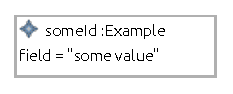
\includegraphics{images/05_library_of_transformations/03_instance_level_transformations/06_data_field_values/data_field_value.pdf}
        \caption{$Im_{DataField}$ with one object and string value ``some value''}
        \label{fig:library_of_transformations:instance_level_transformations:data_field_values:visualisation:ecore}
    \end{subfigure}
    \begin{subfigure}{0.45\textwidth}
        \centering
        % To use this figure in your LaTeX document
% import the package groove/resources/groove2tikz.sty
%
\begin{tikzpicture}[scale=\tikzscale,name prefix=start-]
\node[basic_node] (n0) at (1.595, -0.775) {\ml{\uline{\textit{someId}} : \textbf{Example}\\field = "some value"}};

\end{tikzpicture}

        \caption{$IG_{DataField}$ with one node and string value ``some value''}
        \label{fig:library_of_transformations:instance_level_transformations:data_field_values:visualisation:groove}
    \end{subfigure}
    \caption{Visualisation of the transformation of field values from fields typed by data types}
    \label{fig:library_of_transformations:instance_level_transformations:data_field_values:visualisation}
\end{figure}

The previous sections have shown the instance level transformations of the introduction of all kinds of types and their instances. From this section onward, these types and their instances will be enriched by introducing fields. In this section, the instance level transformation belonging to the transformation of a data field is discussed. The type level transformation for data fields can be found in \cref{subsec:library_of_transformations:type_level_transformations:data_fields}. On the instance level, values for the data fields are introduced.

\begin{defin}[Instance model $Im_{DataField}$]
\label{defin:library_of_transformations:instance_level_transformations:data_field_values:imod_data_field}
Let $Im_{DataField}$ be an instance model typed by $Tm_{DataField}$ (\cref{defin:library_of_transformations:type_level_transformations:data_fields:tmod_data_field}). Define a set $objects$, which represent the objects that will get a value for the field introduced by $Tm_{DataField}$. Furthermore, define a function $obids$ which maps each of these objects to their corresponding identifier and a function $values$, which maps each of these objects to its value for the field introduced by $Tm_{DataField}$. $Im_{DataField}$ is defined as:
\begin{align*}
Object =\ &objects \\
\mathrm{ObjectClass} =\ & \begin{cases}
    (ob, classtype) & \mathrm{if }\ ob \in objects
\end{cases}\\
\mathrm{ObjectId} =\ & \begin{cases}
    (ob, obids(ob)) & \mathrm{if }\ ob \in objects
\end{cases}\\
\mathrm{FieldValue} =\ & \begin{cases}
    ((ob, (classtype, name)), values(ob)) & \mathrm{if }\ ob \in objects
\end{cases} \\
\mathrm{DefaultValue} =\ & \{\}
\end{align*}
\isabellelref{imod_data_field}{Ecore-GROOVE-Mapping-Library.DataFieldValue}
\end{defin}

\begin{thm}[Correctness of $Im_{DataField}$]
\label{defin:library_of_transformations:instance_level_transformations:data_field_values:imod_data_field_correct}
$Im_{DataField}$ (\cref{defin:library_of_transformations:instance_level_transformations:data_field_values:imod_data_field}) is a valid instance model in the sense of \cref{defin:formalisations:ecore_formalisation:instance_models:model_validity}.
\isabellelref{imod_data_field_correct}{Ecore-GROOVE-Mapping-Library.DataFieldValue}
\end{thm}

A visual representation of $Im_{DataField}$ with $objects = \{ob\}$ and $obids(ob) = someId$ can be seen in \cref{fig:library_of_transformations:instance_level_transformations:data_field_values:visualisation:ecore}. In this visualisation, the field value for $ob$ is defined as $values(ob) = \text{``some value''}$. Although this visualisation only shows one object, it is required to define a value for all objects that contain the field. Failing to do so would result in an invalid instance model after it is combined with another model, as the next definition will show. The correctness proof of $Im_{DataField}$ only is already quite involved, but not be included here for conciseness. It can be found as part of the validated Isabelle proofs.

In order to make composing transformation functions possible, $Im_{DataField}$ should be compatible with the instance model it is combined with.

\begin{thm}[Correctness of $\mathrm{combine}(Im, Im_{DataField})$]
\label{defin:library_of_transformations:instance_level_transformations:data_field_values:imod_data_field_combine_correct}
Assume an instance model $Im$ that is valid in the sense of \cref{defin:formalisations:ecore_formalisation:instance_models:model_validity}. Then $Im$ is compatible with $Im_{DataField}$ (in the sense of \cref{defin:transformation_framework:instance_models_and_instance_graphs:combining_instance_models:compatibility}) if:
\begin{itemize}
    \item All requirements of \cref{defin:library_of_transformations:type_level_transformations:data_fields:tmod_data_field_combine_correct} are met, to ensure the combination of the corresponding type models is valid;
    \item The class type on which the field is defined by $Tm_{DataField}$ may not be extended by another class type in the type model corresponding to $Im$;
    \item All of the objects in the set $objects$ must already be objects in $Im$;
    \item All objects typed by the class type on which the field is defined must occur in the set $objects$ and thus have a value in $Im_{DataField}$;
    \item For all of the objects in the set $objects$, the identifier set by $obids$ must be the same identifier as set by $Im$ for that object;
    \item For all objects in set $objects$, the value set by the $values$ function must be valid.
\end{itemize}
\isabellelref{imod_data_field_combine_correct}{Ecore-GROOVE-Mapping-Library.DataFieldValue}
\end{thm}

\begin{proof}
Use \cref{defin:transformation_framework:instance_models_and_instance_graphs:combining_instance_models:imod_combine_merge_correct}. It is possible to show that all assumptions hold. Now we have shown that $\mathrm{combine}(Im, Im_{DataField})$ is consistent in the sense of \cref{defin:formalisations:ecore_formalisation:instance_models:model_validity}.
\end{proof}

As explained earlier, $Im_{DataField}$ needs to introduce values for all objects that are typed by the class type on which the field is defined. This is enforced by the requirements of \cref{defin:library_of_transformations:instance_level_transformations:data_field_values:imod_data_field_combine_correct}. The proof is not included here for conciseness, but can be found as part of the validated proofs in Isabelle.

The definitions and theorems for introducing values for fields of data types within Ecore are now complete. 

\subsubsection{Encoding as edges and nodes}

In the type level transformation of data fields, data fields were encoded in GROOVE as edge types to an primitive type. On the instance level, this edge type will be used and edges will be created to give a value to each node type that has the field defined. The encoding corresponding to $Im_{DataField}$ can then be represented as $IG_{DataField}$, defined in the following definition:

\begin{defin}[Instance graph $IG_{DataField}$]
\label{defin:library_of_transformations:instance_level_transformations:data_field_values:ig_data_field_as_edge_type}
Let $IG_{DataField}$ be the instance graph typed by type graph $TG_{DataField}$ (\cref{defin:library_of_transformations:type_level_transformations:data_fields:tg_data_field_as_edge_type}). Reuse the set $objects$ from $Im_{DataField}$. Moreover, reuse the functions $obids$ and $values$ from $Im_{DataField}$.
The objects in the set $objects$ are converted to nodes in $Im_{DataField}$. For each of these objects, an edge of the encoded field is created. This edge targets a node that corresponds to the value set by $values$ for the corresponding object. Finally, the identity of the objects is defined using $obids$. $IG_{DataField}$ is defined as:
\begin{align*}
N =\ & objects \cup \{values(ob) \mid ob \in objects\} \\
E =\ & \big\{\big(ob, (\mathrm{ns\_\!to\_\!list}(classtype), \langle name \rangle, fieldtype), values(ob)\big) \mid ob \in objects \big\} \\
\mathrm{ident} =\ & \begin{cases}
    (obids(ob), ob) & \mathrm{if }\ ob \in objects
\end{cases}
\end{align*}
with
\begin{align*}
\mathrm{type}_n =\ & \begin{cases}
    (ob, \mathrm{ns\_\!to\_\!list}(classtype)) & \mathrm{if }\ ob \in objects
\end{cases}
\end{align*}
\isabellelref{ig_data_field_as_edge_type}{Ecore-GROOVE-Mapping-Library.DataFieldValue}
\end{defin}

\begin{thm}[Correctness of $IG_{DataField}$]
\label{defin:library_of_transformations:instance_level_transformations:data_field_values:ig_data_field_as_edge_type_correct}
$IG_{DataField}$ (\cref{defin:library_of_transformations:instance_level_transformations:data_field_values:ig_data_field_as_edge_type}) is a valid instance graph in the sense of \cref{defin:formalisations:groove_formalisation:instance_graphs:instance_graph_validity}.
\isabellelref{ig_data_field_as_edge_type_correct}{Ecore-GROOVE-Mapping-Library.DataFieldValue}
\end{thm}

A visual representation of $IG_{DataField}$ with $objects = \{ob\}$ and $obids(ob) = someId$ can be seen in \cref{fig:library_of_transformations:instance_level_transformations:data_field_values:visualisation:groove}. Like the previous visualisation, the field value for $ob$ is defined as $values(ob) = \text{``some value''}$. Although this visualisation only shows one node, it is required to define a value for all nodes typed by the node type corresponding to the field. Failing to do so would result in an invalid instance graph after it is combined with another graph, as the next definition will show. The correctness proof of $IG_{DataField}$ only is already quite involved, but not be included here for conciseness. It can be found as part of the validated Isabelle proofs.

In order to make composing transformation functions possible, $IG_{DataField}$ should be compatible with the instance graph it is combined with.

\begin{thm}[Correctness of $\mathrm{combine}(IG, IG_{DataField})$]
\label{defin:library_of_transformations:instance_level_transformations:data_field_values:ig_data_field_as_edge_type_combine_correct}
Assume an instance graph $IG$ that is valid in the sense of \cref{defin:formalisations:groove_formalisation:instance_graphs:instance_graph_validity}. Then $IG$ is compatible with $IG_{DataField}$ (in the sense of \cref{defin:transformation_framework:instance_models_and_instance_graphs:combining_instance_graphs:compatibility}) if:
\begin{itemize}
    \item All requirements of \cref{defin:library_of_transformations:type_level_transformations:data_fields:tg_data_field_as_edge_type_combine_correct} are met, to ensure the combination of the corresponding type graphs is valid;
    \item The node type on which the corresponding field is defined is not extended by other node types within the type graph corresponding to $IG$;
    \item All nodes in $IG$ that are typed by the node type on which the field is defined are also nodes in $IG_{DataField}$;
    \item For all nodes shared between $IG$ and $IG_{DataField}$, each node must have the same identifier in both $IG$ and $IG_{DataField}$;
    \item For all nodes for which the field is set, the $values$ function must define a valid value;
    \item If an primitive type has incoming or outgoing edge types in the type graph corresponding to $IG$, then the lower multiplicity of these edge types must be 0.
\end{itemize}
\isabellelref{ig_data_field_as_edge_type_combine_correct}{Ecore-GROOVE-Mapping-Library.DataFieldValue}
\end{thm}

\begin{proof}
Use \cref{defin:transformation_framework:instance_models_and_instance_graphs:combining_instance_graphs:ig_combine_merge_correct}. It is possible to show that all assumptions hold. Now we have shown that $\mathrm{combine}(IG, IG_{DataField})$ is valid in the sense of \cref{defin:formalisations:groove_formalisation:instance_graphs:instance_graph_validity}.
\end{proof}

Like the definition for the combination of instance models, the combination of instance graphs also requires the user to set a value for all nodes that are typed by the node type that corresponds to the field type. This is to keep the graph valid.

The next definitions define the transformation function from $Im_{DataField}$ to $IG_{DataField}$:

\begin{defin}[Transformation function $f_{DataField}$]
\label{defin:library_of_transformations:instance_level_transformations:data_field_values:imod_data_field_to_ig_data_field_as_edge_type}
The transformation function $f_{DataField}(Im)$ is defined as:
\begin{align*}
N =\ & Object_{Im} \cup \{values(ob) \mid ob \in Object_{Im}\}  \\
E =\ & \big\{\big(ob, (\mathrm{ns\_\!to\_\!list}(classtype), \langle name \rangle, fieldtype), values(ob)\big) \mid ob \in Object_{Im} \big\} \\
\mathrm{ident} =\ & \begin{cases}
    (obids(ob), ob) & \mathrm{if }\ ob \in Object_{Im}
\end{cases}
\end{align*}
with
\begin{align*}
\mathrm{type}_n =\ & \begin{cases}
    (ob, \mathrm{ns\_\!to\_\!list}(name)) & \mathrm{if }\ ob \in Object_{Im}
\end{cases}
\end{align*}
\isabellelref{imod_data_field_to_ig_data_field_as_edge_type}{Ecore-GROOVE-Mapping-Library.DataFieldValue}
\end{defin}

\begin{thm}[Correctness of $f_{DataField}$]
\label{defin:library_of_transformations:instance_level_transformations:data_field_values:imod_data_field_to_ig_data_field_as_edge_type_func}
$f_{DataField}(Im)$ (\cref{defin:library_of_transformations:instance_level_transformations:data_field_values:imod_data_field_to_ig_data_field_as_edge_type}) is a valid transformation function in the sense of \cref{defin:transformation_framework:instance_models_and_instance_graphs:combining_transformation_functions:transformation_function_instance_model_instance_graph} transforming $Im_{DataField}$ into $IG_{DataField}$.
\isabellelref{imod_data_field_to_ig_data_field_as_edge_type_func}{Ecore-GROOVE-Mapping-Library.DataFieldValue}
\end{thm}

The proof of the correctness of $f_{DataField}$ will not be included here. Instead, it can be found in the validated Isabelle theories.

Finally, to complete the transformation, the transformation function that transforms $IG_{DataField}$ into $Im_{DataField}$ is defined:

\begin{defin}[Transformation function $f'_{DataField}$]
\label{defin:library_of_transformations:instance_level_transformations:data_field_values:ig_data_field_as_edge_type_to_imod_data_field}
The transformation function $f'_{DataField}(IG)$ is defined as:
\begin{align*}
Object =\ &\{\mathrm{src}(e) \mid e \in E_{IG}\} \\
\mathrm{ObjectClass} =\ & \begin{cases}
    (ob, classtype) & \mathrm{if }\ ob \in \{\mathrm{src}(e) \mid e \in E_{IG}\}
\end{cases}\\
\mathrm{ObjectId} =\ & \begin{cases}
    (ob, obids(ob)) & \mathrm{if }\ ob \in \{\mathrm{src}(e) \mid e \in E_{IG}\}
\end{cases}\\
\mathrm{FieldValue} =\ & \begin{cases}
    ((ob, (classtype, name)), values(ob)) & \mathrm{if }\ ob \in \{\mathrm{src}(e) \mid e \in E_{IG}\}
\end{cases} \\
\mathrm{DefaultValue} =\ & \{\}
\end{align*}
\isabellelref{ig_data_field_as_edge_type_to_imod_data_field}{Ecore-GROOVE-Mapping-Library.DataFieldValue}
\end{defin}

\begin{thm}[Correctness of $f'_{DataField}$]
\label{defin:library_of_transformations:instance_level_transformations:data_field_values:ig_data_field_as_edge_type_to_tmod_class_func}
$f'_{DataField}(IG)$ (\cref{defin:library_of_transformations:instance_level_transformations:data_field_values:ig_data_field_as_edge_type_to_imod_data_field}) is a valid transformation function in the sense of \cref{defin:transformation_framework:instance_models_and_instance_graphs:combining_transformation_functions:transformation_function_instance_graph_instance_model} transforming $IG_{DataField}$ into $Im_{DataField}$.
\isabellelref{ig_data_field_as_edge_type_to_imod_data_field_func}{Ecore-GROOVE-Mapping-Library.DataFieldValue}
\end{thm}

Once more, the correctness proof is not included here but can be found in the validated Isabelle proofs of this thesis.
\subsection{Enumeration field values}
\label{subsec:library_of_transformations:instance_level_transformations:enum_field_values}

\begin{figure}
    \centering
    \begin{subfigure}{0.95\textwidth}
        \centering
        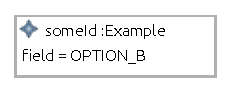
\includegraphics{images/05_library_of_transformations/03_instance_level_transformations/07_enum_field_values/enum_field_value.pdf}
        \caption{$Im_{EnumField}$ with one object and its field referencing enumeration option $OPTION\!\_B$}
        \label{fig:library_of_transformations:instance_level_transformations:enum_field_values:visualisation:ecore}
    \end{subfigure}
    \\
    \begin{subfigure}{0.95\textwidth}
        \centering
        % To use this figure in your LaTeX document
% import the package groove/resources/groove2tikz.sty
%
\begin{tikzpicture}[scale=\tikzscale,name prefix=start-]
\node[basic_node] (n0) at (1.975, -0.185) {\ml{\uline{\textit{someId}} : \textbf{Example}}};
\node[basic_node] (n1) at (5.650, -0.370) {\ml{\uline{\textit{ExistingEnumOptionA}} : \textbf{ExistingEnum\$OPTION\_A}}};
\node[basic_node] (n2) at (1.940, -1.145) {\ml{\uline{\textit{ExistingEnumOptionB}} : \textbf{ExistingEnum\$OPTION\_B}}};
\node[basic_node] (n3) at (5.650, -0.905) {\ml{\uline{\textit{ExistingEnumOptionC}} : \textbf{ExistingEnum\$OPTION\_C}}};

\path[basic_edge](n0.south -| 1.940, -1.145) -- node[lab] {\ml{field}} (n2) ;
\end{tikzpicture}

        \caption{$IG_{EnumFieldNodes}$ with one node and and its edge referencing enumeration option $OPTION\!\_B$}
        \label{fig:library_of_transformations:instance_level_transformations:enum_field_values:visualisation:groove_nodes}
    \end{subfigure}
    \\
    \begin{subfigure}{0.95\textwidth}
        \centering
        % To use this figure in your LaTeX document
% import the package groove/resources/groove2tikz.sty
%
\begin{tikzpicture}[scale=\tikzscale,name prefix=start-]
\node[basic_node] (n0) at (1.975, -0.185) {\ml{\uline{\textit{someId}} : \textbf{Example}}};
\node[basic_node] (n1) at (5.650, -0.370) {\ml{\uline{\textit{ExistingEnumOptionA}} : \textbf{ExistingEnum}\\\textit{OPTION\_A}}};
\node[basic_node] (n2) at (1.940, -1.125) {\ml{\uline{\textit{ExistingEnumOptionB}} : \textbf{ExistingEnum}\\\textit{OPTION\_B}}};
\node[basic_node] (n3) at (5.650, -0.905) {\ml{\uline{\textit{ExistingEnumOptionC}} : \textbf{ExistingEnum}\\\textit{OPTION\_C}}};

\path[basic_edge](n0.south -| 1.940, -1.125) -- node[lab] {\ml{field}} (n2) ;
\end{tikzpicture}

        \caption{$IG_{EnumFieldFlags}$ with one node and its edge referencing enumeration option $OPTION\!\_B$}
        \label{fig:library_of_transformations:instance_level_transformations:enum_field_values:visualisation:groove_flags}
    \end{subfigure}
    \caption{Visualisation of the transformation of field values from fields typed by enumeration types}
    \label{fig:library_of_transformations:instance_level_transformations:enum_field_values:visualisation}
\end{figure}

In this section, the instance level transformation belonging to the transformation of an enumeration field is discussed. The type level transformation for enumeration fields can be found in \cref{subsec:library_of_transformations:type_level_transformations:enum_fields}. On the instance level, values for the enumeration fields are introduced.

\begin{defin}[Instance model $Im_{EnumField}$]
\label{defin:library_of_transformations:instance_level_transformations:enum_field_values:imod_enum_field}
Let $Im_{EnumField}$ be an instance model typed by $Tm_{EnumField}$ (\cref{defin:library_of_transformations:type_level_transformations:enum_fields:tmod_enum_field}). Define a set $objects$, which represent the objects that will get a value for the field introduced by $Tm_{EnumField}$. Furthermore, define a function $obids$ which maps each of these objects to their corresponding identifier and a function $values$, which maps each of these objects to its value for the field introduced by $Tm_{EnumField}$. $Im_{EnumField}$ is defined as:
\begin{align*}
Object =\ &objects \\
\mathrm{ObjectClass} =\ & \begin{cases}
    (ob, classtype) & \mathrm{if }\ ob \in objects
\end{cases}\\
\mathrm{ObjectId} =\ & \begin{cases}
    (ob, obids(ob)) & \mathrm{if }\ ob \in objects
\end{cases}\\
\mathrm{FieldValue} =\ & \begin{cases}
    \Big((ob, (classtype, name)), \big[\type{enum}, (enumid, values(ob))\big]\Big) & \mathrm{if }\ ob \in objects
\end{cases} \\
\mathrm{DefaultValue} =\ & \{\}
\end{align*}
\isabellelref{imod_enum_field}{Ecore-GROOVE-Mapping-Library.EnumFieldValue}
\end{defin}

\begin{thm}[Correctness of $Im_{EnumField}$]
\label{defin:library_of_transformations:instance_level_transformations:enum_field_values:imod_enum_field_correct}
$Im_{EnumField}$ (\cref{defin:library_of_transformations:instance_level_transformations:enum_field_values:imod_enum_field}) is a valid instance model in the sense of \cref{defin:formalisations:ecore_formalisation:instance_models:model_validity}.
\isabellelref{imod_enum_field_correct}{Ecore-GROOVE-Mapping-Library.EnumFieldValue}
\end{thm}

A visual representation of $Im_{EnumField}$ with $objects = \{ob\}$ and $obids(ob) = someId$ can be seen in \cref{fig:library_of_transformations:instance_level_transformations:enum_field_values:visualisation:ecore}. In this visualisation, the field value for $ob$ is defined as $values(ob) = OPTION\!\_B$. Although this visualisation only shows one object, it is required to define a value for all objects that contain the field. Failing to do so would result in an invalid instance model after it is combined with another model, as the next definition will show. The correctness proof of $Im_{EnumField}$ only is quite involved, but not be included here for conciseness. It can be found as part of the validated Isabelle proofs.

In order to make composing transformation functions possible, $Im_{EnumField}$ should be compatible with the instance model it is combined with.

\begin{thm}[Correctness of $\mathrm{combine}(Im, Im_{EnumField})$]
\label{defin:library_of_transformations:instance_level_transformations:enum_field_values:imod_enum_field_combine_correct}
Assume an instance model $Im$ that is valid in the sense of \cref{defin:formalisations:ecore_formalisation:instance_models:model_validity}. Then $Im$ is compatible with $Im_{EnumField}$ (in the sense of \cref{defin:transformation_framework:instance_models_and_instance_graphs:combining_instance_models:compatibility}) if:
\begin{itemize}
    \item All requirements of \cref{defin:library_of_transformations:type_level_transformations:enum_fields:tmod_enum_field_combine_correct} are met, to ensure the combination of the corresponding type models is valid;
    \item The class type on which the field is defined by $Tm_{EnumField}$ may not be extended by another class type in the type model corresponding to $Im$;
    \item All of the objects in the set $objects$ must already be objects in $Im$;
    \item All objects typed by the class type on which the field is defined must occur in the set $objects$ and thus have a value in $Im_{EnumField}$;
    \item For all of the objects in the set $objects$, the identifier set by $obids$ must be the same identifier as set by $Im$ for that object;
    \item For all objects in set $objects$, the value set by the $values$ function must be valid.
\end{itemize}
\isabellelref{imod_enum_field_combine_correct}{Ecore-GROOVE-Mapping-Library.EnumFieldValue}
\end{thm}

\begin{proof}
Use \cref{defin:transformation_framework:instance_models_and_instance_graphs:combining_instance_models:imod_combine_merge_correct}. It is possible to show that all assumptions hold. Now we have shown that $\mathrm{combine}(Im, Im_{EnumField})$ is consistent in the sense of \cref{defin:formalisations:ecore_formalisation:instance_models:model_validity}.
\end{proof}

As explained earlier, $Im_{EnumField}$ needs to introduce values for all objects that are typed by the class type on which the field is defined. This is enforced by the requirements of \cref{defin:library_of_transformations:instance_level_transformations:enum_field_values:imod_enum_field_combine_correct}. The proof is not included here for conciseness, but can be found as part of the validated proofs in Isabelle.

The definitions and theorems for introducing values for fields of data types within Ecore are now complete. 

\subsubsection{Encoding as edges and nodes with a node type encoded enumeration type}

As discussed in \cref{subsec:library_of_transformations:type_level_transformations:enum_fields}, there are two different encodings for a field typed by an enumeration type. These correspond to the two different encodings of the enumeration type itself. On the instance level, these encodings also need to be distinguished. The first encoding of the values assumes that the enumeration is encoded using node types. The encoding corresponding to $Im_{EnumField}$ is then represented as $IG_{EnumFieldNodes}$, defined in the following definition:

\begin{defin}[Instance graph $IG_{EnumFieldNodes}$]
\label{defin:library_of_transformations:instance_level_transformations:enum_field_values:ig_enum_as_node_types_field_as_edge_type}
Let $IG_{EnumFieldNodes}$ be the instance graph typed by type graph $TG_{EnumFieldNodes}$ (\cref{defin:library_of_transformations:type_level_transformations:enum_fields:tg_enum_as_node_types_field_as_edge_type}). Reuse the set $objects$ from $Im_{EnumField}$. Moreover, reuse the functions $obids$ and $values$ from $Im_{EnumField}$. Furthermore, define $enumob$ to be the function that maps an enumeration value to an internal node identity. Similarly, define $enumids$ as the function that maps an enumeration value to its explicit node id.

Within $IG_{EnumFieldNodes}$, the objects in the set $objects$ are converted to nodes in $Im_{EnumField}$. For each of these objects, an edge of the encoded field is created. This edge targets a node that corresponds to the value set by $values$ for the corresponding object. Furthermore, the identity of the objects is defined using $obids$. Finally, ensure that the instances of the enumeration values exist and encode them in the same way as $IG_{EnumNodes}$ (\cref{defin:library_of_transformations:instance_level_transformations:enumeration_values:ig_enum_as_node_types}). $IG_{EnumFieldNodes}$ is defined as:
\begin{align*}
N =\ & objects \cup \{enumob(v) \mid v \in enumvalues \} \\
E =\ & \big\{\big(ob, (\mathrm{ns\_\!to\_\!list}(classtype), \langle name \rangle, \mathrm{ns\_\!to\_\!list}(enumid)), enumob(values(ob))\big) \mid ob \in objects \big\} \\
\mathrm{ident} =\ & \begin{cases}
    (obids(ob), ob) & \mathrm{if }\ ob \in objects\\
    (enumids(v), enumob(v)) & \mathrm{if }\ v \in enumvalues
\end{cases}
\end{align*}
with
\begin{align*}
\mathrm{type}_n =\ & \begin{cases}
    (ob, \mathrm{ns\_\!to\_\!list}(classtype)) & \mathrm{if }\ ob \in objects\\
    (enumob(v), \mathrm{ns\_\!to\_\!list}(enumid) \append \langle v \rangle) & \mathrm{if }\ v \in enumvalues
\end{cases}
\end{align*}
\isabellelref{ig_enum_as_node_types_field_as_edge_type}{Ecore-GROOVE-Mapping-Library.EnumFieldValue}
\end{defin}

\begin{thm}[Correctness of $IG_{EnumFieldNodes}$]
\label{defin:library_of_transformations:instance_level_transformations:enum_field_values:ig_enum_as_node_types_field_as_edge_type_correct}
$IG_{EnumFieldNodes}$ (\cref{defin:library_of_transformations:instance_level_transformations:enum_field_values:ig_enum_as_node_types_field_as_edge_type}) is a valid instance graph in the sense of \cref{defin:formalisations:groove_formalisation:instance_graphs:instance_graph_validity}.
\isabellelref{ig_enum_as_node_types_field_as_edge_type_correct}{Ecore-GROOVE-Mapping-Library.EnumFieldValue}
\end{thm}

A visual representation of $IG_{EnumFieldNodes}$ with $objects = \{ob\}$ and $obids(ob) = someId$ can be seen in \cref{fig:library_of_transformations:instance_level_transformations:enum_field_values:visualisation:groove_nodes}. Like the previous visualisation, the field value for $ob$ is defined as $values(ob) = OPTION\!\_B$. Although this visualisation only shows one node, it is required to define a value for all nodes that are typed by the node type corresponding to the field. Failing to do so would result in an invalid instance graph after it is combined with another graph, as the next definition will show. The correctness proof of $IG_{EnumFieldNodes}$ only is quite involved, but not be included here for conciseness. It can be found as part of the validated Isabelle proofs.

In order to make composing transformation functions possible, $IG_{EnumFieldNodes}$ should be compatible with the instance graph it is combined with.

\begin{thm}[Correctness of $\mathrm{combine}(IG, IG_{EnumFieldNodes})$]
\label{defin:library_of_transformations:instance_level_transformations:enum_field_values:ig_enum_as_node_types_field_as_edge_type_combine_correct}
Assume an instance graph $IG$ that is valid in the sense of \cref{defin:formalisations:groove_formalisation:instance_graphs:instance_graph_validity}. Then $IG$ is compatible with $IG_{EnumFieldNodes}$ (in the sense of \cref{defin:transformation_framework:instance_models_and_instance_graphs:combining_instance_graphs:compatibility}) if:
\begin{itemize}
    \item All requirements of \cref{defin:library_of_transformations:type_level_transformations:enum_fields:tg_enum_as_node_types_field_as_edge_type_combine_correct} are met, to ensure the combination of the corresponding type graphs is valid;
    \item The node type on which the corresponding field is defined is not extended by other node types within the type graph corresponding to $IG$;
    \item All nodes in $IG$ that are typed by the node type on which the field is defined are also nodes in $IG_{EnumFieldNodes}$;
    \item All nodes in $IG_{EnumFieldNodes}$ that encode the values of the corresponding enumeration type are also nodes in $IG$;
    \item For all nodes shared between $IG$ and $IG_{EnumFieldNodes}$, each node must have the same identifier in both $IG$ and $IG_{EnumFieldNodes}$;
    \item For all nodes for which the field is set, the $values$ function must define a valid value.
\end{itemize}
\isabellelref{ig_enum_as_node_types_field_as_edge_type_combine_correct}{Ecore-GROOVE-Mapping-Library.EnumFieldValue}
\end{thm}

\begin{proof}
Use \cref{defin:transformation_framework:instance_models_and_instance_graphs:combining_instance_graphs:ig_combine_merge_correct}. It is possible to show that all assumptions hold. Now we have shown that $\mathrm{combine}(IG, IG_{EnumFieldNodes})$ is valid in the sense of \cref{defin:formalisations:groove_formalisation:instance_graphs:instance_graph_validity}.
\end{proof}

Like the definition for the combination of instance models, the combination of instance graphs also requires the user to set a value for all nodes that are typed by the node type that corresponds to the field type. This is to keep the graph valid.

The next definitions define the transformation function from $Im_{EnumField}$ to $IG_{EnumFieldNodes}$:

\begin{defin}[Transformation function $f_{EnumFieldNodes}$]
\label{defin:library_of_transformations:instance_level_transformations:enum_field_values:imod_enum_field_to_ig_enum_as_node_types_field_as_edge_type}
The transformation function $f_{EnumFieldNodes}(Im)$ is defined as:
\begin{align*}
N =\ & Object_{Im} \cup \{enumob(ob) \mid v \in enumvalues\}  \\
E =\ & \big\{\big(ob, (\mathrm{ns\_\!to\_\!list}(classtype), \langle name \rangle, \mathrm{ns\_\!to\_\!list}(enumid)), enumob(values(ob))\big) \mid \\&ob \in Object_{Im} \big\} \\
\mathrm{ident} =\ & \begin{cases}
    (obids(ob), ob) & \mathrm{if }\ ob \in Object_{Im}\\
    (enumids(v), enumob(v)) & \mathrm{if }\ v \in enumvalues
\end{cases}
\end{align*}
with
\begin{align*}
\mathrm{type}_n =\ & \begin{cases}
    (ob, \mathrm{ns\_\!to\_\!list}(classtype)) & \mathrm{if }\ ob \in Object_{Im}\\
    (enumob(v), \mathrm{ns\_\!to\_\!list}(enumid) \append \langle v \rangle) & \mathrm{if }\ v \in enumvalues
\end{cases}
\end{align*}
\isabellelref{imod_enum_field_to_ig_enum_as_node_types_field_as_edge_type}{Ecore-GROOVE-Mapping-Library.EnumFieldValue}
\end{defin}

\begin{thm}[Correctness of $f_{EnumFieldNodes}$]
\label{defin:library_of_transformations:instance_level_transformations:enum_field_values:imod_enum_field_to_ig_enum_as_node_types_field_as_edge_type_func}
$f_{EnumFieldNodes}(Im)$ (\cref{defin:library_of_transformations:instance_level_transformations:enum_field_values:imod_enum_field_to_ig_enum_as_node_types_field_as_edge_type}) is a valid transformation function in the sense of \cref{defin:transformation_framework:instance_models_and_instance_graphs:combining_transformation_functions:transformation_function_instance_model_instance_graph} transforming $Im_{EnumField}$ into $IG_{EnumFieldNodes}$.
\isabellelref{imod_enum_field_to_ig_enum_as_node_types_field_as_edge_type_func}{Ecore-GROOVE-Mapping-Library.EnumFieldValue}
\end{thm}

The proof of the correctness of $f_{EnumFieldNodes}$ will not be included here. Instead, it can be found in the validated Isabelle theories.

Finally, to complete the transformation, the transformation function that transforms $IG_{EnumFieldNodes}$ into $Im_{EnumField}$ is defined:

\begin{defin}[Transformation function $f'_{EnumFieldNodes}$]
\label{defin:library_of_transformations:instance_level_transformations:enum_field_values:ig_enum_as_node_types_field_as_edge_type_to_imod_enum_field}
The transformation function $f'_{EnumFieldNodes}(IG)$ is defined as:
\begin{align*}
Object =\ &\{\mathrm{src}(e) \mid e \in E_{IG}\} \\
\mathrm{ObjectClass} =\ & \begin{cases}
    (ob, name) & \mathrm{if }\ ob \in \{\mathrm{src}(e) \mid e \in E_{IG}\}
\end{cases}\\
\mathrm{ObjectId} =\ & \begin{cases}
    (ob, obids(ob)) & \mathrm{if }\ ob \in \{\mathrm{src}(e) \mid e \in E_{IG}\}
\end{cases}\\
\mathrm{FieldValue} =\ & \begin{cases}
    \Big((ob, (classtype, name)), \big(\type{enum}, (enumid, values(ob))\big)\Big) & \mathrm{if }\ ob \in \{\mathrm{src}(e) \mid e \in E_{IG}\}
\end{cases} \\
\mathrm{DefaultValue} =\ & \{\}
\end{align*}
\isabellelref{ig_enum_as_node_types_field_as_edge_type_to_imod_enum_field}{Ecore-GROOVE-Mapping-Library.EnumFieldValue}
\end{defin}

\begin{thm}[Correctness of $f'_{EnumFieldNodes}$]
\label{defin:library_of_transformations:instance_level_transformations:enum_field_values:ig_enum_as_node_types_field_as_edge_type_to_tmod_class_func}
$f'_{EnumFieldNodes}(IG)$ (\cref{defin:library_of_transformations:instance_level_transformations:enum_field_values:ig_enum_as_node_types_field_as_edge_type_to_imod_enum_field}) is a valid transformation function in the sense of \cref{defin:transformation_framework:instance_models_and_instance_graphs:combining_transformation_functions:transformation_function_instance_graph_instance_model} transforming $IG_{EnumFieldNodes}$ into $Im_{EnumField}$.
\isabellelref{ig_enum_as_node_types_field_as_edge_type_to_imod_enum_field_func}{Ecore-GROOVE-Mapping-Library.EnumFieldValue}
\end{thm}

Once more, the correctness proof is not included here but can be found in the validated Isabelle proofs of this thesis.

\subsubsection{Encoding as edges and nodes with a flag encoded enumeration type}

The second possible encoding of the values assumes that the enumeration is encoded using flags. The encoding corresponding to $Im_{EnumField}$ is then represented as $IG_{EnumFieldFlags}$, defined in the following definition:

\begin{defin}[Instance graph $IG_{EnumFieldFlags}$]
\label{defin:library_of_transformations:instance_level_transformations:enum_field_values:ig_enum_as_flags_field_as_edge_type}
Let $IG_{EnumFieldFlags}$ be the instance graph typed by type graph $TG_{EnumFieldFlags}$ (\cref{defin:library_of_transformations:type_level_transformations:enum_fields:tg_enum_as_flags_field_as_edge_type}). Reuse the set $objects$ from $Im_{EnumField}$. Moreover, reuse the functions $obids$ and $values$ from $Im_{EnumField}$. Furthermore, define $enumob$ to be the function that maps an enumeration value to an internal node identity. Similarly, define $enumids$ as the function that maps an enumeration value to its explicit node id.

Within $IG_{EnumFieldFlags}$, the objects in the set $objects$ are converted to nodes in $Im_{EnumField}$. For each of these objects, an edge of the encoded field is created. This edge targets a node that corresponds to the value set by $values$ for the corresponding object. Furthermore, the identity of the objects is defined using $obids$. Finally, ensure that the instances of the enumeration values exist and encode them in the same way as $IG_{EnumFlags}$ (\cref{defin:library_of_transformations:instance_level_transformations:enumeration_values:ig_enum_as_flags}). $IG_{EnumFieldFlags}$ is defined as:
\begin{align*}
N =\ & objects \cup \{enumob(v) \mid v \in enumvalues \} \\
E =\ & \big\{\big(ob, (\mathrm{ns\_\!to\_\!list}(classtype), \langle name \rangle, \mathrm{ns\_\!to\_\!list}(enumid)), enumob(values(ob))\big) \mid ob \in objects \big\} \\
\mathrm{ident} =\ & \begin{cases}
    (obids(ob), ob) & \mathrm{if }\ ob \in objects\\
    (enumids(v), enumob(v)) & \mathrm{if }\ v \in enumvalues
\end{cases}
\end{align*}
with
\begin{align*}
\mathrm{type}_n =\ & \begin{cases}
    (ob, \mathrm{ns\_\!to\_\!list}(classtype)) & \mathrm{if }\ ob \in objects\\
    (enumob(v), \mathrm{ns\_\!to\_\!list}(enumid)) & \mathrm{if }\ v \in enumvalues
\end{cases}
\end{align*}
\isabellelref{ig_enum_as_flags_field_as_edge_type}{Ecore-GROOVE-Mapping-Library.EnumFieldValue}
\end{defin}

\begin{thm}[Correctness of $IG_{EnumFieldFlags}$]
\label{defin:library_of_transformations:instance_level_transformations:enum_field_values:ig_enum_as_flags_field_as_edge_type_correct}
$IG_{EnumFieldFlags}$ (\cref{defin:library_of_transformations:instance_level_transformations:enum_field_values:ig_enum_as_flags_field_as_edge_type}) is a valid instance graph in the sense of \cref{defin:formalisations:groove_formalisation:instance_graphs:instance_graph_validity}.
\isabellelref{ig_enum_as_flags_field_as_edge_type_correct}{Ecore-GROOVE-Mapping-Library.EnumFieldValue}
\end{thm}

A visual representation of $IG_{EnumFieldFlags}$ with $objects = \{ob\}$ and $obids(ob) = someId$ can be seen in \cref{fig:library_of_transformations:instance_level_transformations:enum_field_values:visualisation:groove_flags}. It does not differ much from the previous encoding, except that the values of the enumeration type are shown as flags on the nodes instead of using seperate types. The formal definition is therefore very similar, except for the definition of $\mathrm{type}_n$. Although this visualisation only shows one node, it is required to define a value for all nodes that are typed by the node type corresponding to the field. Failing to do so would, once more, result in an invalid instance graph after it is combined with another graph. The correctness proof of $IG_{EnumFieldFlags}$ only is quite involved, but not be included here for conciseness. It can be found as part of the validated Isabelle proofs.

In order to make composing transformation functions possible, $IG_{EnumFieldFlags}$ should be compatible with the instance graph it is combined with.

\begin{thm}[Correctness of $\mathrm{combine}(IG, IG_{EnumFieldFlags})$]
\label{defin:library_of_transformations:instance_level_transformations:enum_field_values:ig_enum_as_flags_field_as_edge_type_combine_correct}
Assume an instance graph $IG$ that is valid in the sense of \cref{defin:formalisations:groove_formalisation:instance_graphs:instance_graph_validity}. Then $IG$ is compatible with $IG_{EnumFieldFlags}$ (in the sense of \cref{defin:transformation_framework:instance_models_and_instance_graphs:combining_instance_graphs:compatibility}) if:
\begin{itemize}
    \item All requirements of \cref{defin:library_of_transformations:type_level_transformations:enum_fields:tg_enum_as_flags_field_as_edge_type_combine_correct} are met, to ensure the combination of the corresponding type graphs is valid;
    \item The node type on which the corresponding field is defined is not extended by other node types within the type graph corresponding to $IG$;
    \item All nodes in $IG$ that are typed by the node type on which the field is defined are also nodes in $IG_{EnumFieldFlags}$;
    \item All nodes in $IG_{EnumFieldFlags}$ that encode the values of the corresponding enumeration type are also nodes in $IG$;
    \item For all nodes shared between $IG$ and $IG_{EnumFieldFlags}$, each node must have the same identifier in both $IG$ and $IG_{EnumFieldFlags}$;
    \item For all nodes for which the field is set, the $values$ function must define a valid value.
\end{itemize}
\isabellelref{ig_enum_as_flags_field_as_edge_type_combine_correct}{Ecore-GROOVE-Mapping-Library.EnumFieldValue}
\end{thm}

\begin{proof}
Use \cref{defin:transformation_framework:instance_models_and_instance_graphs:combining_instance_graphs:ig_combine_merge_correct}. It is possible to show that all assumptions hold. Now we have shown that $\mathrm{combine}(IG, IG_{EnumFieldFlags})$ is valid in the sense of \cref{defin:formalisations:groove_formalisation:instance_graphs:instance_graph_validity}.
\end{proof}

The next definitions define the transformation function from $Im_{EnumField}$ to $IG_{EnumFieldFlags}$:

\begin{defin}[Transformation function $f_{EnumFieldFlags}$]
\label{defin:library_of_transformations:instance_level_transformations:enum_field_values:imod_enum_field_to_ig_enum_as_flags_field_as_edge_type}
The transformation function $f_{EnumFieldFlags}(Im)$ is defined as:
\begin{align*}
N =\ & Object_{Im} \cup \{enumob(ob) \mid v \in enumvalues\}  \\
E =\ & \big\{\big(ob, (\mathrm{ns\_\!to\_\!list}(classtype), \langle name \rangle, \mathrm{ns\_\!to\_\!list}(enumid)), enumob(values(ob))\big) \mid \\&ob \in Object_{Im} \big\} \\
\mathrm{ident} =\ & \begin{cases}
    (obids(ob), ob) & \mathrm{if }\ ob \in Object_{Im}\\
    (enumids(v), enumob(v)) & \mathrm{if }\ v \in enumvalues
\end{cases}
\end{align*}
with
\begin{align*}
\mathrm{type}_n =\ & \begin{cases}
    (ob, \mathrm{ns\_\!to\_\!list}(classtype)) & \mathrm{if }\ ob \in Object_{Im}\\
    (enumob(v), \mathrm{ns\_\!to\_\!list}(enumid)) & \mathrm{if }\ v \in enumvalues
\end{cases}
\end{align*}
\isabellelref{imod_enum_field_to_ig_enum_as_flags_field_as_edge_type}{Ecore-GROOVE-Mapping-Library.EnumFieldValue}
\end{defin}

\begin{thm}[Correctness of $f_{EnumFieldFlags}$]
\label{defin:library_of_transformations:instance_level_transformations:enum_field_values:imod_enum_field_to_ig_enum_as_flags_field_as_edge_type_func}
$f_{EnumFieldFlags}(Im)$ (\cref{defin:library_of_transformations:instance_level_transformations:enum_field_values:imod_enum_field_to_ig_enum_as_flags_field_as_edge_type}) is a valid transformation function in the sense of \cref{defin:transformation_framework:instance_models_and_instance_graphs:combining_transformation_functions:transformation_function_instance_model_instance_graph} transforming $Im_{EnumField}$ into $IG_{EnumFieldFlags}$.
\isabellelref{imod_enum_field_to_ig_enum_as_flags_field_as_edge_type_func}{Ecore-GROOVE-Mapping-Library.EnumFieldValue}
\end{thm}

The proof of the correctness of $f_{EnumFieldFlags}$ will not be included here. Instead, it can be found in the validated Isabelle theories.

Finally, to complete the transformation, the transformation function that transforms $IG_{EnumFieldFlags}$ into $Im_{EnumField}$ is defined:

\begin{defin}[Transformation function $f'_{EnumFieldFlags}$]
\label{defin:library_of_transformations:instance_level_transformations:enum_field_values:ig_enum_as_flags_field_as_edge_type_to_imod_enum_field}
The transformation function $f'_{EnumFieldFlags}(IG)$ is defined as:
\begin{align*}
Object =\ &\{\mathrm{src}(e) \mid e \in E_{IG}\} \\
\mathrm{ObjectClass} =\ & \begin{cases}
    (ob, classtype) & \mathrm{if }\ ob \in \{\mathrm{src}(e) \mid e \in E_{IG}\}
\end{cases}\\
\mathrm{ObjectId} =\ & \begin{cases}
    (ob, obids(ob)) & \mathrm{if }\ ob \in \{\mathrm{src}(e) \mid e \in E_{IG}\}
\end{cases}\\
\mathrm{FieldValue} =\ & \begin{cases}
    \Big((ob, (classtype, name)), \big[\type{enum}, (enumid, values(ob))\big]\Big) & \mathrm{if }\ ob \in \{\mathrm{src}(e) \mid e \in E_{IG}\}
\end{cases} \\
\mathrm{DefaultValue} =\ & \{\}
\end{align*}
\isabellelref{ig_enum_as_flags_field_as_edge_type_to_imod_enum_field}{Ecore-GROOVE-Mapping-Library.EnumFieldValue}
\end{defin}

\begin{thm}[Correctness of $f'_{EnumFieldFlags}$]
\label{defin:library_of_transformations:instance_level_transformations:enum_field_values:ig_enum_as_flags_field_as_edge_type_to_tmod_class_func}
$f'_{EnumFieldFlags}(IG)$ (\cref{defin:library_of_transformations:instance_level_transformations:enum_field_values:ig_enum_as_flags_field_as_edge_type_to_imod_enum_field}) is a valid transformation function in the sense of \cref{defin:transformation_framework:instance_models_and_instance_graphs:combining_transformation_functions:transformation_function_instance_graph_instance_model} transforming $IG_{EnumFieldFlags}$ into $Im_{EnumField}$.
\isabellelref{ig_enum_as_flags_field_as_edge_type_to_imod_enum_field_func}{Ecore-GROOVE-Mapping-Library.EnumFieldValue}
\end{thm}

Once more, the correctness proof is not included here but can be found in the validated Isabelle proofs of this thesis.
\subsection{Nullable class field values}
\label{subsec:library_of_transformations:instance_level_transformations:nullable_class_field_values}

\begin{figure}
    \centering
    \begin{subfigure}{0.95\textwidth}
        \centering
        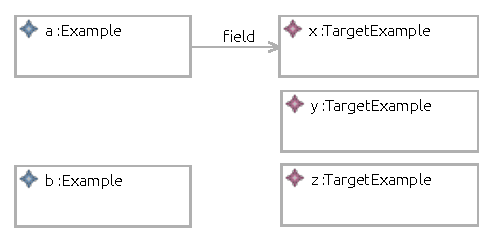
\includegraphics{images/05_library_of_transformations/03_instance_level_transformations/08_nullable_class_field_values/nullable_class_field_value.pdf}
        \caption{$Im_{NullableClassField}$ with examples of different nodes with different values for $\type{field}$}
        \label{fig:library_of_transformations:instance_level_transformations:nullable_class_field_values:visualisation:ecore}
    \end{subfigure}
    \\
    \begin{subfigure}{0.95\textwidth}
        \centering
        % To use this figure in your LaTeX document
% import the package groove/resources/groove2tikz.sty
%
\begin{tikzpicture}[scale=\tikzscale,name prefix=start-]
\node[basic_node] (n0) at (1.795, -0.405) {\ml{\uline{\textit{a}} : \textbf{Example}}};
\node[basic_node] (n1) at (1.795, -0.805) {\ml{\uline{\textit{b}} : \textbf{Example}}};
\node[basic_node] (n2) at (3.750, -0.440) {\ml{\uline{\textit{x}} : \textbf{TargetExample}}};
\node[basic_node] (n3) at (3.745, -0.815) {\ml{\uline{\textit{y}} : \textbf{TargetExample}}};
\node[basic_node] (n4) at (3.740, -1.205) {\ml{\uline{\textit{z}} : \textbf{TargetExample}}};

\path[basic_edge](n0.east |- 3.750, -0.440) -- node[lab] {\ml{field}} (n2) ;
\end{tikzpicture}

        \caption{$IG_{NullableClassField}$ with examples of different nodes with different values for $\type{field}$}
        \label{fig:library_of_transformations:instance_level_transformations:nullable_class_field_values:visualisation:groove}
    \end{subfigure}
    \caption{Visualisation of the transformation of field values from fields typed by nullable class types}
    \label{fig:library_of_transformations:instance_level_transformations:nullable_class_field_values:visualisation}
\end{figure}

This section introduces the instance level transformation belonging to the transformation of a nullable class field. The type level transformation for nullable class fields can be found in \cref{subsec:library_of_transformations:type_level_transformations:nullable_class_fields}. On the instance level, values for these fields are introduced.

\begin{defin}[Instance model $Im_{NullableClassField}$]
\label{defin:library_of_transformations:instance_level_transformations:nullable_class_field_values:imod_nullable_class_field}
Let $Im_{NullableClassField}$ be an instance model typed by $Tm_{NullableClassField}$ (\cref{defin:library_of_transformations:type_level_transformations:nullable_class_fields:tmod_nullable_class_field}). Define disjoint sets $valobjects$ and $nilobjects$. The objects in $valobjects$ will get a proper class value for the field introduced by $Tm_{NullableClassField}$, while the objects in $nilobjects$ get a $\type{nil}$ value for the same field. Furthermore, define a function $obids$ which maps each of these objects to their corresponding identifier and a function $values$, which maps the objects in $valobjects$ to its value for the field introduced by $Tm_{NullableClassField}$. $Im_{NullableClassField}$ is defined as:
\begin{align*}
Object =\ &nilobjects \cup valobjects \cup \{ values(ob) \mid ob \in valobjects \} \\
\mathrm{ObjectClass} =\ & \begin{cases}
    (ob, classtype) & \mathrm{if }\ ob \in nilobjects \cup valobjects\\
    (ob, fieldtype) & \mathrm{if }\ ob \in \{ values(ob) \mid ob \in valobjects \}
\end{cases}\\
\mathrm{ObjectId} =\ & \begin{cases}
    (ob, obids(ob)) & \mathrm{if }\ ob \in objects
\end{cases}\\
\mathrm{FieldValue} =\ & \begin{cases}
    ((ob, (classtype, name)), \type{nil}) & \mathrm{if }\ ob \in nilobjects\\
    ((ob, (classtype, name)), [\type{obj}, values(ob)]) & \mathrm{if }\ ob \in valobjects
\end{cases} \\
\mathrm{DefaultValue} =\ & \{\}
\end{align*}
\isabellelref{imod_nullable_class_field}{Ecore-GROOVE-Mapping-Library.NullableClassFieldValue}
\end{defin}

\begin{thm}[Correctness of $Im_{NullableClassField}$]
\label{defin:library_of_transformations:instance_level_transformations:nullable_class_field_values:imod_nullable_class_field_correct}
$Im_{NullableClassField}$ (\cref{defin:library_of_transformations:instance_level_transformations:nullable_class_field_values:imod_nullable_class_field}) is a valid instance model in the sense of \cref{defin:formalisations:ecore_formalisation:instance_models:model_validity}.
\isabellelref{imod_nullable_class_field_correct}{Ecore-GROOVE-Mapping-Library.NullableClassFieldValue}
\end{thm}

A visual representation of $Im_{NullableClassField}$ with $valobjects = \{ob_a\}$ and $nilobjects = \{ob_b\}$ can be seen in \cref{fig:library_of_transformations:instance_level_transformations:nullable_class_field_values:visualisation:ecore}. In this visualisation, the field value for $ob_a$ is defined as $values(ob_a) = ob_x$. Furthermore, the value for $ob_b$ is $\type{nil}$, because it occurs within the set $nilobjects$. Like the previous transformations for field values, the value needs to be set for all objects that are typed by the class type corresponding to the field. Failing to do so would result in an invalid instance model after it is combined with another model, as the next definition will show. The correctness proof of $Im_{NullableClassField}$ only is already quite involved, but not be included here for conciseness. It can be found as part of the validated Isabelle proofs.

In order to make composing transformation functions possible, $Im_{NullableClassField}$ should be compatible with the instance model it is combined with.

\begin{thm}[Correctness of $\mathrm{combine}(Im, Im_{NullableClassField})$]
\label{defin:library_of_transformations:instance_level_transformations:nullable_class_field_values:imod_nullable_class_field_combine_correct}
Assume an instance model $Im$ that is valid in the sense of \cref{defin:formalisations:ecore_formalisation:instance_models:model_validity}. Then $Im$ is compatible with $Im_{NullableClassField}$ (in the sense of \cref{defin:transformation_framework:instance_models_and_instance_graphs:combining_instance_models:compatibility}) if:
\begin{itemize}
    \item All requirements of \cref{defin:library_of_transformations:type_level_transformations:nullable_class_fields:tmod_nullable_class_field_combine_correct} are met, to ensure the combination of the corresponding type models is valid;
    \item The class type on which the field is defined by $Tm_{NullableClassField}$ may not be extended by another class type in the type model corresponding to $Im$;
    \item All of the objects in the sets $nilobjects$ and $valobjects$ must already be objects in $Im$;
    \item All of the objects referenced by the objects in the set $valobjects$ must already be objects in $Im$;
    \item All objects typed by the class type on which the field is defined must occur in the set $nilobjects \cup valobjects$ and thus have a value in $Im_{NullableClassField}$;
    \item For all of the objects in the set $objects$, the identifier set by $obids$ must be the same identifier as set by $Im$ for that object;
    \item The sets $valobjects$ and $nilobjects$ must be disjoint, each object only gets a proper class value or a nil value, not both;
    \item For all objects in set $valobjects$, the value set by the $values$ function must be valid.
\end{itemize}
\isabellelref{imod_nullable_class_field_combine_correct}{Ecore-GROOVE-Mapping-Library.NullableClassFieldValue}
\end{thm}

\begin{proof}
Use \cref{defin:transformation_framework:instance_models_and_instance_graphs:combining_instance_models:imod_combine_merge_correct}. It is possible to show that all assumptions hold. Now we have shown that $\mathrm{combine}(Im, Im_{NullableClassField})$ is consistent in the sense of \cref{defin:formalisations:ecore_formalisation:instance_models:model_validity}.
\end{proof}

As explained earlier, $Im_{NullableClassField}$ needs to introduce values for all objects that are typed by the class type on which the field is defined. This is enforced by the requirements of \cref{defin:library_of_transformations:instance_level_transformations:nullable_class_field_values:imod_nullable_class_field_combine_correct}. The proof is not included here for conciseness, but can be found as part of the validated proofs in Isabelle.

The definitions and theorems for introducing values for fields of data types within Ecore are now complete. 

\subsubsection{Encoding as edges and nodes}

In the type level transformation of nullable class fields, nullable class fields were encoded in GROOVE as edge types to a corresponding encoded node type. On the instance level, this edge type will be used and edges will be created to give a value to each node type that has the field defined. The encoding corresponding to $Im_{NullableClassField}$ can then be represented as $IG_{NullableClassField}$, defined in the following definition:

\begin{defin}[Instance graph $IG_{NullableClassField}$]
\label{defin:library_of_transformations:instance_level_transformations:nullable_class_field_values:ig_nullable_class_field_as_edge_type}
Let $IG_{NullableClassField}$ be the instance graph typed by type graph $TG_{NullableClassField}$ (\cref{defin:library_of_transformations:type_level_transformations:nullable_class_fields:tg_nullable_class_field_as_edge_type}). Reuse the sets $nilobjects$ and $valobjects$ from $Im_{NullableClassField}$. Moreover, reuse the functions $obids$ and $values$ from $Im_{NullableClassField}$.

The objects in the sets $nilobjects$ and $valobjects$ are converted to nodes in $Im_{NullableClassField}$. For each of these objects, an edge of the encoded field is created. This edge targets a node that corresponds to the value set by $values$ for the corresponding object in $valobjects$. The outgoing multiplicity of the edge type created by $TG_{NullableClassField}$ is $0..1$, such that the objects in $nilobjects$ do not need to have this edge, representing the absence of a value. Finally, the identity of the objects is defined using $obids$. $IG_{NullableClassField}$ is defined as:
\begin{align*}
N =\ & nilobjects \cup valobjects \cup \{values(ob) \mid ob \in valobjects\} \\
E =\ & \big\{\big(ob, (\mathrm{ns\_\!to\_\!list}(classtype), \langle name \rangle, \mathrm{ns\_\!to\_\!list}(fieldtype)), values(ob)\big) \mid ob \in valobjects \big\} \\
\mathrm{ident} =\ & \begin{cases}
    (obids(ob), ob) & \mathrm{if }\ ob \in objects
\end{cases}
\end{align*}
with
\begin{align*}
\mathrm{type}_n =\ & \begin{cases}
    (ob, \mathrm{ns\_\!to\_\!list}(classtype)) & \mathrm{if }\ ob \in nilobjects \cup valobjects\\
    (ob, \mathrm{ns\_\!to\_\!list}(fieldtype)) & \mathrm{if }\ ob \in \{values(ob) \mid ob \in valobjects\}
\end{cases}
\end{align*}
\isabellelref{ig_nullable_class_field_as_edge_type}{Ecore-GROOVE-Mapping-Library.NullableClassFieldValue}
\end{defin}

\begin{thm}[Correctness of $IG_{NullableClassField}$]
\label{defin:library_of_transformations:instance_level_transformations:nullable_class_field_values:ig_nullable_class_field_as_edge_type_correct}
$IG_{NullableClassField}$ (\cref{defin:library_of_transformations:instance_level_transformations:nullable_class_field_values:ig_nullable_class_field_as_edge_type}) is a valid instance graph in the sense of \cref{defin:formalisations:groove_formalisation:instance_graphs:instance_graph_validity}.
\isabellelref{ig_nullable_class_field_as_edge_type_correct}{Ecore-GROOVE-Mapping-Library.NullableClassFieldValue}
\end{thm}

A visual representation of $IG_{NullableClassField}$ with $valobjects = \{ob_a\}$ and $nilobjects = \{ob_b\}$ can be seen in \cref{fig:library_of_transformations:instance_level_transformations:nullable_class_field_values:visualisation:groove}. Like the previous visualisation, the field value for $ob_a$ is defined as $values(ob_a) = ob_x$. Since $ob_b$ was in the set $nilobjects$, no edge has been created for this node. Like the previous field encodings, one needs to set the values for the field for all objects of the encoded class type at once. Failing to do so would result in an invalid instance graph after it is combined with another graph, as the next definition will show. The correctness proof of $IG_{NullableClassField}$ only is already quite involved, but not be included here for conciseness. It can be found as part of the validated Isabelle proofs.

In order to make composing transformation functions possible, $IG_{NullableClassField}$ should be compatible with the instance graph it is combined with.

\begin{thm}[Correctness of $\mathrm{combine}(IG, IG_{NullableClassField})$]
\label{defin:library_of_transformations:instance_level_transformations:nullable_class_field_values:ig_nullable_class_field_as_edge_type_combine_correct}
Assume an instance graph $IG$ that is valid in the sense of \cref{defin:formalisations:groove_formalisation:instance_graphs:instance_graph_validity}. Then $IG$ is compatible with $IG_{NullableClassField}$ (in the sense of \cref{defin:transformation_framework:instance_models_and_instance_graphs:combining_instance_graphs:compatibility}) if:
\begin{itemize}
    \item All requirements of \cref{defin:library_of_transformations:type_level_transformations:nullable_class_fields:tg_nullable_class_field_as_edge_type_combine_correct} are met, to ensure the combination of the corresponding type graphs is valid;
    \item The node type on which the corresponding field is defined is not extended by other node types within the type graph corresponding to $IG$;
    \item All nodes in $IG$ are also nodes in $IG_{NullableClassField}$;
    \item For all nodes shared between $IG$ and $IG_{NullableClassField}$, each node must have the same identifier in both $IG$ and $IG_{NullableClassField}$;
    \item The sets $valobjects$ and $nilobjects$ must be disjoint, each node gets either one edge to another node, or no edge at all;
    \item For all nodes for which the field is set, the $values$ function must define a valid value.
\end{itemize}
\isabellelref{ig_nullable_class_field_as_edge_type_combine_correct}{Ecore-GROOVE-Mapping-Library.NullableClassFieldValue}
\end{thm}

\begin{proof}
Use \cref{defin:transformation_framework:instance_models_and_instance_graphs:combining_instance_graphs:ig_combine_merge_correct}. It is possible to show that all assumptions hold. Now we have shown that $\mathrm{combine}(IG, IG_{NullableClassField})$ is valid in the sense of \cref{defin:formalisations:groove_formalisation:instance_graphs:instance_graph_validity}.
\end{proof}

The next definitions define the transformation function from $Im_{NullableClassField}$ to $IG_{NullableClassField}$:

\begin{defin}[Transformation function $f_{NullableClassField}$]
\label{defin:library_of_transformations:instance_level_transformations:nullable_class_field_values:imod_nullable_class_field_to_ig_nullable_class_field_as_edge_type}
The transformation function $f_{NullableClassField}(Im)$ is defined as:
\begin{align*}
N =\ & Object_{Im}  \\
E =\ & \big\{\big(ob, (\mathrm{ns\_\!to\_\!list}(classtype), \langle name \rangle, \mathrm{ns\_\!to\_\!list}(fieldtype)), values(ob)\big) \mid\\&ob \in Object_{Im} \land ob \in valobjects \big\} \\
\mathrm{ident} =\ & \begin{cases}
    (obids(ob), ob) & \mathrm{if }\ ob \in Object_{Im}
\end{cases}
\end{align*}
with
\begin{align*}
\mathrm{type}_n =\ & \begin{cases}
    (ob, \mathrm{ns\_\!to\_\!list}(name)) & \mathrm{if }\ ob \in Object_{Im} \land ob \in nilobjects \cup valobjects\\
    (ob, \mathrm{ns\_\!to\_\!list}(name)) & \mathrm{if }\ ob \in Object_{Im} \land ob \in \{values(ob) \mid ob \in valobjects\} 
\end{cases}
\end{align*}
\isabellelref{imod_nullable_class_field_to_ig_nullable_class_field_as_edge_type}{Ecore-GROOVE-Mapping-Library.NullableClassFieldValue}
\end{defin}

\begin{thm}[Correctness of $f_{NullableClassField}$]
\label{defin:library_of_transformations:instance_level_transformations:nullable_class_field_values:imod_nullable_class_field_to_ig_nullable_class_field_as_edge_type_func}
$f_{NullableClassField}(Im)$ (\cref{defin:library_of_transformations:instance_level_transformations:nullable_class_field_values:imod_nullable_class_field_to_ig_nullable_class_field_as_edge_type}) is a valid transformation function in the sense of \cref{defin:transformation_framework:instance_models_and_instance_graphs:combining_transformation_functions:transformation_function_instance_model_instance_graph} transforming $Im_{NullableClassField}$ into $IG_{NullableClassField}$.
\isabellelref{imod_nullable_class_field_to_ig_nullable_class_field_as_edge_type_func}{Ecore-GROOVE-Mapping-Library.NullableClassFieldValue}
\end{thm}

The proof of the correctness of $f_{NullableClassField}$ will not be included here. Instead, it can be found in the validated Isabelle theories.

Finally, to complete the transformation, the transformation function that transforms $IG_{NullableClassField}$ into $Im_{NullableClassField}$ is defined:

\begin{defin}[Transformation function $f'_{NullableClassField}$]
\label{defin:library_of_transformations:instance_level_transformations:nullable_class_field_values:ig_nullable_class_field_as_edge_type_to_imod_nullable_class_field}
The transformation function $f'_{NullableClassField}(IG)$ is defined as:
\begin{align*}
Object =\ &N_{IG} \\
\mathrm{ObjectClass} =\ & \begin{cases}
    (ob, classtype) & \mathrm{if }\ ob \in N_{IG} \land ob \in nilobjects \cup valobjects \\
    (ob, fieldtype) & \mathrm{if }\ ob \in N_{IG} \land ob \in \{values(ob) \mid ob \in valobjects\}
\end{cases}\\
\mathrm{ObjectId} =\ & \begin{cases}
    (ob, obids(ob)) & \mathrm{if }\ ob \in N_{IG}
\end{cases}\\
\mathrm{FieldValue} =\ & \begin{cases}
    ((ob, (classtype, name)), \type{nil}) & \mathrm{if }\ ob \in N_{IG} \land ob \in nilobjects\\
    ((ob, (classtype, name)), [\type{obj}, values(ob)]) & \mathrm{if }\ ob \in N_{IG} \land ob \in valobjects
\end{cases} \\
\mathrm{DefaultValue} =\ & \{\}
\end{align*}
\isabellelref{ig_nullable_class_field_as_edge_type_to_imod_nullable_class_field}{Ecore-GROOVE-Mapping-Library.NullableClassFieldValue}
\end{defin}

\begin{thm}[Correctness of $f'_{NullableClassField}$]
\label{defin:library_of_transformations:instance_level_transformations:nullable_class_field_values:ig_nullable_class_field_as_edge_type_to_tmod_class_func}
$f'_{NullableClassField}(IG)$ (\cref{defin:library_of_transformations:instance_level_transformations:nullable_class_field_values:ig_nullable_class_field_as_edge_type_to_imod_nullable_class_field}) is a valid transformation function in the sense of \cref{defin:transformation_framework:instance_models_and_instance_graphs:combining_transformation_functions:transformation_function_instance_graph_instance_model} transforming $IG_{NullableClassField}$ into $Im_{NullableClassField}$.
\isabellelref{ig_nullable_class_field_as_edge_type_to_imod_nullable_class_field_func}{Ecore-GROOVE-Mapping-Library.NullableClassFieldValue}
\end{thm}

Once more, the correctness proof is not included here but can be found in the validated Isabelle proofs of this thesis.
%\writingtask{Write about the proper class sequence field value transformation}
\subsection{Contained class set field values}
\label{subsec:library_of_transformations:instance_level_transformations:contained_class_set_field_values}

\begin{figure}
    \centering
    \begin{subfigure}{0.95\textwidth}
        \centering
        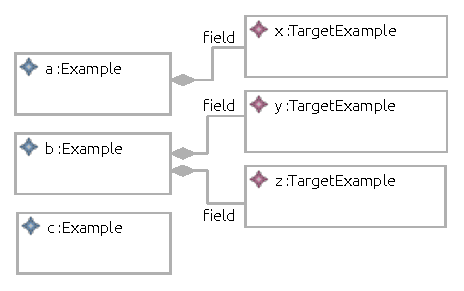
\includegraphics{images/05_library_of_transformations/03_instance_level_transformations/10_contained_class_set_field_values/contained_class_set_field_value.pdf}
        \caption{$Im_{ContainedClassSetField}$ with examples of different nodes with different values for $\type{field}$}
        \label{fig:library_of_transformations:instance_level_transformations:contained_class_set_field_values:visualisation:ecore}
    \end{subfigure}
    \\
    \begin{subfigure}{0.95\textwidth}
        \centering
        % To use this figure in your LaTeX document
% import the package groove/resources/groove2tikz.sty
%
\begin{tikzpicture}[scale=\tikzscale,name prefix=start-]
\node[basic_node] (n0) at (1.805, -0.645) {\ml{\uline{\textit{a}} : \textbf{Example}}};
\node[basic_node] (n1) at (1.805, -1.035) {\ml{\uline{\textit{b}} : \textbf{Example}}};
\node[basic_node] (n2) at (3.750, -0.440) {\ml{\uline{\textit{x}} : \textbf{TargetExample}}};
\node[basic_node] (n3) at (3.745, -0.815) {\ml{\uline{\textit{y}} : \textbf{TargetExample}}};
\node[basic_node] (n4) at (3.740, -1.205) {\ml{\uline{\textit{z}} : \textbf{TargetExample}}};
\node[basic_node] (n5) at (1.800, -1.410) {\ml{\uline{\textit{c}} : \textbf{Example}}};

\path[basic_edge] (n0)  -- node[lab] {\ml{field}} (n2) ;
\path[basic_edge] (n1)  -- node[lab] {\ml{field}} (n4) ;
\path[basic_edge] (n1)  -- node[lab] {\ml{field}} (n3) ;
\end{tikzpicture}

        \caption{$IG_{ContainedClassSetField}$ with examples of different nodes with different values for $\type{field}$}
        \label{fig:library_of_transformations:instance_level_transformations:contained_class_set_field_values:visualisation:groove}
    \end{subfigure}
    \caption{Visualisation of the transformation of field values from containment fields typed by a set of a proper class type}
    \label{fig:library_of_transformations:instance_level_transformations:contained_class_set_field_values:visualisation}
\end{figure}

This section introduces the instance level transformation belonging to the transformation of a containment field of a set of a proper class type. The type level transformation belonging to these fields can be found in \cref{subsec:library_of_transformations:type_level_transformations:contained_class_set_fields}. On the instance level, values for these fields are introduced.

\begin{defin}[Instance model $Im_{ContainedClassSetField}$]
\label{defin:library_of_transformations:instance_level_transformations:contained_class_set_field_values:imod_contained_class_set_field}
Let $Im_{ContainedClassSetField}$ be an instance model typed by $Tm_{ContainedClassSetField}$ (\cref{defin:library_of_transformations:type_level_transformations:contained_class_set_fields:tmod_contained_class_set_field}). Define a set $objects$, which represent the objects that will get a value for the field introduced by $Tm_{DataField}$. Furthermore, define a function $obids$ which maps each of these objects to their corresponding identifier and a function $values$, which maps each of these objects to its value for the field introduced by $Tm_{DataField}$. Please note that $values$ returns a set of objects, as the field allows for this. $Im_{DataField}$ is defined as:
\begin{align*}
Object =\ &objects \cup \bigg(\bigcup_{ob \in objects} values(ob)\bigg)\\
\mathrm{ObjectClass} =\ & \begin{cases}
    (ob, classtype) & \mathrm{if }\ ob \in objects\\
    (ob, containedtype) & \mathrm{if }\ ob \in \bigcup_{ob \in objects} values(ob)
\end{cases}\\
\mathrm{ObjectId} =\ & \begin{cases}
    (ob, obids(ob)) & \mathrm{if }\ ob \in objects
\end{cases}\\
\mathrm{FieldValue} =\ & \begin{cases}
    \Big((ob, (classtype, name)), \big[\type{setof}, \langle [\type{obj}, ob] \mid ob \in values(ob) \rangle\big]\Big) & \mathrm{if }\ ob \in objects
\end{cases} \\
\mathrm{DefaultValue} =\ & \{\}
\end{align*}
\isabellelref{imod_contained_class_set_field}{Ecore-GROOVE-Mapping-Library.ContainedClassSetFieldValue}
\end{defin}

\begin{thm}[Correctness of $Im_{ContainedClassSetField}$]
\label{defin:library_of_transformations:instance_level_transformations:contained_class_set_field_values:imod_contained_class_set_field_correct}
$Im_{ContainedClassSetField}$ (\cref{defin:library_of_transformations:instance_level_transformations:contained_class_set_field_values:imod_contained_class_set_field}) is a valid instance model in the sense of \cref{defin:formalisations:ecore_formalisation:instance_models:model_validity}.
\isabellelref{imod_contained_class_set_field_correct}{Ecore-GROOVE-Mapping-Library.ContainedClassSetFieldValue}
\end{thm}

A visual representation of $Im_{ContainedClassSetField}$ with $objects = \{ob_a, ob_b, ob_c\}$ can be seen in \cref{fig:library_of_transformations:instance_level_transformations:contained_class_set_field_values:visualisation:ecore}. This example is typed by $Tm_{ContainedClassSetField}$ in \cref{fig:library_of_transformations:type_level_transformations:contained_class_set_fields:visualisation:ecore}. In this visualisation, the field value for $ob_a$ is defined as $values(ob_a) = \{ob_x\}$. Furthermore, the value for $ob_b$ is $values(ob_a) = \{ob_y, ob_z\}$. Finally, the value for $ob_c$ is $values(ob_c) = \{\}$, which is allowed because the lower bound of the multiplicity is set 0 by the example. Like the previous transformations for field values, the value needs to be set for all objects that are typed by the class type corresponding to the field. Failing to do so would result in an invalid instance model after it is combined with another model, as the next definition will show. The correctness proof of $Im_{ContainedClassSetField}$ only is already quite involved, but not be included here for conciseness. It can be found as part of the validated Isabelle proofs.

In order to make composing transformation functions possible, $Im_{ContainedClassSetField}$ should be compatible with the instance model it is combined with.

\begin{thm}[Correctness of $\mathrm{combine}(Im, Im_{ContainedClassSetField})$]
\label{defin:library_of_transformations:instance_level_transformations:contained_class_set_field_values:imod_contained_class_set_field_combine_correct}
Assume an instance model $Im$ that is valid in the sense of \cref{defin:formalisations:ecore_formalisation:instance_models:model_validity}. Then $Im$ is compatible with $Im_{ContainedClassSetField}$ (in the sense of \cref{defin:transformation_framework:instance_models_and_instance_graphs:combining_instance_models:compatibility}) if:
\begin{itemize}
    \item All requirements of \cref{defin:library_of_transformations:type_level_transformations:contained_class_set_fields:tmod_contained_class_set_field_combine_correct} are met, to ensure the combination of the corresponding type models is valid;
    \item The class type on which the field is defined by $Tm_{ContainedClassSetField}$ may not be extended by another class type in the type model corresponding to $Im$;
    \item The contained type and the class type cannot be the same, e.g. $classtype \neq containedtype$.
    \item All of the objects in the set $objects$ must already be objects in $Im$;
    \item All of the referenced objects cannot be objects in $Im$, they are newly introduced by $Im_{ContainedClassSetField}$;
    \item All objects typed by the class type on which the field is defined must occur in the set $objects$ and thus have a value in $Im_{ContainedClassSetField}$;
    \item For all of the objects in the set $objects$, the identifier set by $obids$ must be the same identifier as set by $Im$ for that object;
    \item The object ids for the newly introduced objects must be unique with respect to each other and all other objects within $Im$;
    \item For all objects in set $valobjects$, the value set by the $values$ function must be valid and the amount of elements in each value must be within the multiplicity $mul$.
\end{itemize}
\isabellelref{imod_contained_class_set_field_combine_correct}{Ecore-GROOVE-Mapping-Library.ContainedClassSetFieldValue}
\end{thm}

\begin{proof}
Use \cref{defin:transformation_framework:instance_models_and_instance_graphs:combining_instance_models:imod_combine_merge_correct}. It is possible to show that all assumptions hold. Now we have shown that $\mathrm{combine}(Im, Im_{ContainedClassSetField})$ is consistent in the sense of \cref{defin:formalisations:ecore_formalisation:instance_models:model_validity}.
\end{proof}

Please note that all objects referenced by any objects via this field are newly created. They may not exist on the existing model. This is enforced to ensure that the containment relations of objects remain acyclic, which is needed to keep the instance model valid. The proof is not included here for conciseness, but can be found as part of the validated proofs in Isabelle.

The definitions and theorems for introducing values for fields of data types within Ecore are now complete. 

\subsubsection{Encoding as edges and nodes}

In the type level transformation of contained class set fields, a single containment edge type was introduced to encode the values for the containment field. On the instance level, the values for each object will be encoded using this edge type. The encoding corresponding to $Im_{ContainedClassSetField}$ can then be represented as $IG_{ContainedClassSetField}$, defined in the following definition:

\begin{defin}[Instance graph $IG_{ContainedClassSetField}$]
\label{defin:library_of_transformations:instance_level_transformations:contained_class_set_field_values:ig_contained_class_set_field_as_edge_type}
Let $IG_{ContainedClassSetField}$ be the instance graph typed by type graph $TG_{ContainedClassSetField}$ (\cref{defin:library_of_transformations:type_level_transformations:contained_class_set_fields:tg_contained_class_set_field_as_edge_type}). Reuse the set $objects$ from $Im_{ContainedClassSetField}$. Moreover, reuse the functions $obids$ and $values$ from $Im_{ContainedClassSetField}$.

The objects in the set $objects$ are converted to nodes in $Im_{ContainedClassSetField}$. For each of these objects, a edge is created for each referenced object within the value of that field. Each of these edges targets an node that encodes an object that was referenced by the value. Finally, the identity of the objects is defined using $obids$. $IG_{ContainedClassSetField}$ is defined as:
\begin{align*}
N =\ & objects \cup \bigg(\bigcup_{ob \in objects} values(ob)\bigg)\\
E =\ & \bigcup_{ob \in objects} \big\{\big(ob, (\mathrm{ns\_\!to\_\!list}(classtype), \langle name \rangle, \mathrm{ns\_\!to\_\!list}(containedtype)), v\big) \mid v \in values(ob) \big\} \\
\mathrm{ident} =\ & \begin{cases}
    (obids(ob), ob) & \mathrm{if }\ ob \in objects \cup \Big(\bigcup_{ob \in objects} values(ob)\Big)
\end{cases}
\end{align*}
with
\begin{align*}
\mathrm{type}_n =\ & \begin{cases}
    (ob, \mathrm{ns\_\!to\_\!list}(classtype)) & \mathrm{if }\ ob \in objects\\
    (v, \mathrm{ns\_\!to\_\!list}(containedtype)) & \mathrm{if }\ v \in \bigcup_{ob \in objects} values(ob)
\end{cases}
\end{align*}
\isabellelref{ig_contained_class_set_field_as_edge_type}{Ecore-GROOVE-Mapping-Library.ContainedClassSetFieldValue}
\end{defin}

\begin{thm}[Correctness of $IG_{ContainedClassSetField}$]
\label{defin:library_of_transformations:instance_level_transformations:contained_class_set_field_values:ig_contained_class_set_field_as_edge_type_correct}
$IG_{ContainedClassSetField}$ (\cref{defin:library_of_transformations:instance_level_transformations:contained_class_set_field_values:ig_contained_class_set_field_as_edge_type}) is a valid instance graph in the sense of \cref{defin:formalisations:groove_formalisation:instance_graphs:instance_graph_validity}.
\isabellelref{ig_contained_class_set_field_as_edge_type_correct}{Ecore-GROOVE-Mapping-Library.ContainedClassSetFieldValue}
\end{thm}

A visual representation of $IG_{ContainedClassSetField}$ with $objects = \{ob_a, ob_b, ob_c\}$ can be seen in \cref{fig:library_of_transformations:instance_level_transformations:contained_class_set_field_values:visualisation:groove}. This example is typed by $TG_{ContainedClassSetField}$ in \cref{fig:library_of_transformations:type_level_transformations:contained_class_set_fields:visualisation:groove}. In this visualisation, the field value for $ob_a$ is defined as $values(ob_a) = \{ob_x\}$. Furthermore, the value for $ob_b$ is $values(ob_a) = \{ob_y, ob_z\}$. Finally, the value for $ob_c$ is $values(ob_c) = \{\}$. Like the previous field encodings, one needs to set the values for the field for all objects of the encoded class type at once. Failing to do so would result in an invalid instance graph after it is combined with another graph, as the next definition will show. The correctness proof of $IG_{ContainedClassSetField}$ only is already quite involved, but not be included here for conciseness. It can be found as part of the validated Isabelle proofs.

In order to make composing transformation functions possible, $IG_{ContainedClassSetField}$ should be compatible with the instance graph it is combined with.

\begin{thm}[Correctness of $\mathrm{combine}(IG, IG_{ContainedClassSetField})$]
\label{defin:library_of_transformations:instance_level_transformations:contained_class_set_field_values:ig_contained_class_set_field_as_edge_type_combine_correct}
Assume an instance graph $IG$ that is valid in the sense of \cref{defin:formalisations:groove_formalisation:instance_graphs:instance_graph_validity}. Then $IG$ is compatible with $IG_{ContainedClassSetField}$ (in the sense of \cref{defin:transformation_framework:instance_models_and_instance_graphs:combining_instance_graphs:compatibility}) if:
\begin{itemize}
    \item All requirements of \cref{defin:library_of_transformations:type_level_transformations:contained_class_set_fields:tg_contained_class_set_field_as_edge_type_combine_correct} are met, to ensure the combination of the corresponding type graphs is valid;
    \item The node type on which the corresponding field is defined is not extended by other node types within the type graph corresponding to $IG$;
    \item The contained type and the class type cannot be the same, e.g. $classtype \neq containedtype$.
    \item All nodes in $objects$ are also nodes in $IG_{ContainedClassSetField}$;
    \item All nodes referenced by the nodes in $objects$ are not already nodes in $IG_{ContainedClassSetField}$, e.g. the nodes referenced by values are newly introduced;
    \item All nodes typed by the node type on which the field is defined must occur in the set $objects$ and thus have a value in $IG_{ContainedClassSetField}$;
    \item The object ids for the newly introduced objects must be unique with respect to each other and all other objects within $IG$;
    \item For all nodes shared between $IG$ and $IG_{ContainedClassSetField}$, each node must have the same identifier in both $IG$ and $IG_{ContainedClassSetField}$;
    \item For all nodes in set $objects$, the value set by the $values$ function must be valid and the amount of elements in each value must be within the multiplicity $mul$.
\end{itemize}
\isabellelref{ig_contained_class_set_field_as_edge_type_combine_correct}{Ecore-GROOVE-Mapping-Library.ContainedClassSetFieldValue}
\end{thm}

\begin{proof}
Use \cref{defin:transformation_framework:instance_models_and_instance_graphs:combining_instance_graphs:ig_combine_merge_correct}. It is possible to show that all assumptions hold. Now we have shown that $\mathrm{combine}(IG, IG_{ContainedClassSetField})$ is valid in the sense of \cref{defin:formalisations:groove_formalisation:instance_graphs:instance_graph_validity}.
\end{proof}

The next definitions define the transformation function from $Im_{ContainedClassSetField}$ to \\$IG_{ContainedClassSetField}$:

\begin{defin}[Transformation function $f_{ContainedClassSetField}$]
\label{defin:library_of_transformations:instance_level_transformations:contained_class_set_field_values:imod_contained_class_set_field_to_ig_contained_class_set_field_as_edge_type}
The transformation function $f_{ContainedClassSetField}(Im)$ is defined as:
\begin{align*}
N =\ & Object_{Im}\\
E =\ & \bigcup_{ob \in Object_{Im} \land ob \in objects} \big\{\big(ob, (\mathrm{ns\_\!to\_\!list}(classtype), \langle name \rangle, \mathrm{ns\_\!to\_\!list}(containedtype)), v\big) \mid\\&\qquad\qquad\qquad\qquad\qquad v \in values(ob) \big\} \\
\mathrm{ident} =\ & \begin{cases}
    (obids(ob), ob) & \mathrm{if }\ ob \in Object_{Im}
\end{cases}
\end{align*}
with
\begin{align*}
\mathrm{type}_n =\ & \begin{cases}
    (ob, \mathrm{ns\_\!to\_\!list}(classtype)) & \mathrm{if }\ ob \in Object_{Im} \land ob \in objects\\
    (v, \mathrm{ns\_\!to\_\!list}(containedtype)) & \mathrm{if }\ v \in \bigcup_{ob \in Object_{Im} \land ob \in objects} values(ob)
\end{cases}
\end{align*}
\isabellelref{imod_contained_class_set_field_to_ig_contained_class_set_field_as_edge_type}{Ecore-GROOVE-Mapping-Library.ContainedClassSetFieldValue}
\end{defin}

\begin{thm}[Correctness of $f_{ContainedClassSetField}$]
\label{defin:library_of_transformations:instance_level_transformations:contained_class_set_field_values:imod_contained_class_set_field_to_ig_contained_class_set_field_as_edge_type_func}
$f_{ContainedClassSetField}(Im)$ (\cref{defin:library_of_transformations:instance_level_transformations:contained_class_set_field_values:imod_contained_class_set_field_to_ig_contained_class_set_field_as_edge_type}) is a valid transformation function in the sense of \cref{defin:transformation_framework:instance_models_and_instance_graphs:combining_transformation_functions:transformation_function_instance_model_instance_graph} transforming $Im_{ContainedClassSetField}$ into $IG_{ContainedClassSetField}$.
\isabellelref{imod_contained_class_set_field_to_ig_contained_class_set_field_as_edge_type_func}{Ecore-GROOVE-Mapping-Library.ContainedClassSetFieldValue}
\end{thm}

The proof of the correctness of $f_{ContainedClassSetField}$ will not be included here. Instead, it can be found in the validated Isabelle theories.

Finally, to complete the transformation, the transformation function that transforms \\$IG_{ContainedClassSetField}$ into $Im_{ContainedClassSetField}$ is defined:

\begin{defin}[Transformation function $f'_{ContainedClassSetField}$]
\label{defin:library_of_transformations:instance_level_transformations:contained_class_set_field_values:ig_contained_class_set_field_as_edge_type_to_imod_contained_class_set_field}
The transformation function $f'_{ContainedClassSetField}(IG)$ is defined as:
\begin{align*}
Object =\ &N_{IG} \\
\mathrm{ObjectClass} =\ & \begin{cases}
    (ob, classtype) & \mathrm{if }\ ob \in N_{IG} \land ob \in objects\\
    (ob, containedtype) & \mathrm{if }\ ob \in N_{IG} \land ob \in \bigcup_{ob \in objects} values(ob)
\end{cases}\\
\mathrm{ObjectId} =\ & \begin{cases}
    (ob, obids(ob)) & \mathrm{if }\ ob \in N_{IG}
\end{cases}\\
\mathrm{FieldValue} =\ & \begin{cases}
    \Big((ob, (classtype, name)), \big[\type{setof}, \langle [\type{obj}, ob] \mid ob \in values(ob) \rangle\big]\Big) & \mathrm{if }\ ob \in N_{IG}\ \land\\&\quad ob \in objects
\end{cases} \\
\mathrm{DefaultValue} =\ & \{\}
\end{align*}
\isabellelref{ig_contained_class_set_field_as_edge_type_to_imod_contained_class_set_field}{Ecore-GROOVE-Mapping-Library.ContainedClassSetFieldValue}
\end{defin}

\begin{thm}[Correctness of $f'_{ContainedClassSetField}$]
\label{defin:library_of_transformations:instance_level_transformations:contained_class_set_field_values:ig_contained_class_set_field_as_edge_type_to_tmod_class_func}
$f'_{ContainedClassSetField}(IG)$ (\cref{defin:library_of_transformations:instance_level_transformations:contained_class_set_field_values:ig_contained_class_set_field_as_edge_type_to_imod_contained_class_set_field}) is a valid transformation function in the sense of \cref{defin:transformation_framework:instance_models_and_instance_graphs:combining_transformation_functions:transformation_function_instance_graph_instance_model} transforming $IG_{ContainedClassSetField}$ into $Im_{ContainedClassSetField}$.
\isabellelref{ig_contained_class_set_field_as_edge_type_to_imod_contained_class_set_field_func}{Ecore-GROOVE-Mapping-Library.ContainedClassSetFieldValue}
\end{thm}

Once more, the correctness proof is not included here but can be found in the validated Isabelle proofs of this thesis.